\documentclass[11pt]{article}

\usepackage{a4wide}
\usepackage[utf8]{inputenc}
\usepackage[russian]{babel}
\usepackage{graphicx}
\usepackage{amsmath}
\usepackage{amsthm} 
\usepackage{amsfonts}
\usepackage{amssymb}
\usepackage{subcaption}
\usepackage{upgreek}
\usepackage{dsfont}
\begin{document}
	\newtheorem{theorem}{Теорема}
	\newtheorem{opr}{Определение}
	\newtheorem{utv}{Утверждение}
	\thispagestyle{empty}
	
	\begin{center}
		\ \vspace{-3cm}
		
		
\includegraphics[width=0.5\textwidth]{msu.eps}\\
		{\scshape Московский государственный университет имени М.~В.~Ломоносова}\\
		Факультет вычислительной математики и кибернетики\\
		Кафедра системного анализа
		
		\vfill
		
		{\LARGE Отчёт по практикуму}
		
		\vspace{1cm}
		
		{\Huge\bfseries <<Стохастический анализ и моделирование>>}
	\end{center}
	
	\vspace{1cm}
	
	\begin{flushright}
		\large
		\textit{Студент 415 группы}\\
		А.\,В.~Бабаев
		
		\vspace{5mm}
		
		\textit{Научный руководитель}\\
		 доцент, к.ф.-м.н. С.\,Н.~Смирнов
	\end{flushright}
	
	\vfill
	
	\begin{center}
		Москва, 2021
	\end{center}
	
	\newpage
	\tableofcontents
	\newpage
	\section{Задание №1}
	\subsection{Постановка задачи}
	\begin{itemize}
		\item [1.]{Реализовать генератор схемы Бернулли с заданной вероятностью успеха $p$. На основе генератора схемы Бернулли построить датчик биномиального распределения. }
		\item [2.]{Реализовать генератор геометрического распределения. Проверить для данного распределения свойство отсутствия памяти.}
		\item [3.]{Рассмотреть игру в орлянку - бесконечную последовательность независимых испытаний с бросанием правильной монеты. Выигрыш $S_n$ определяется как сумма по всем $n$ испытаниям значений 1 и -1 в зависимости от выпавшей стороны. Проиллюстрировать (в виде ломаной) поведение нормированной суммы $Y(i) = S_i / \sqrt{n}$, как функцию от номера испытания $i = 1\dots n$ для одной отдельно взятой траектории. Дать теоретическую оценку для $Y(n)$ при $ n \rightarrow \infty.$  }
	\end{itemize}
    \subsection{Решение}
    \subsubsection{Генератор схемы Бернулли. Датчик для биномиального распределения}
    \begin{opr}
    	{Схемой Бернулли с заданной вероятностью успеха $p$ называется эксперимент, состоящий из серии испытаний, удовлетворяющих следующим условиям:}
    	\begin{itemize}
    		\item [1.]{Отсутствие взаимного влияния в испытаниях (одно на другое не оказывает влияния).}
    		\item [2.]{Воспроизводимость. Однородные испытания проводятся в схожих условиях (не одинаковых).}
    		\item [3.]{Существует признак, которые реализуется (успех) с вероятностью $p$, или не реализуется (неуспех) с вероятностью $1-p$.}
    	\end{itemize}
    \end{opr}
    
    \begin{opr}
    	Говорят, что случайная величина $X$ имеет распределение Бернулли, если она принимает значение 1 с вероятностью $p$ и 0 с вероятностью $1 - p$. Обозначение: $X \thicksim Bern(p).$
    \end{opr}
	
	{Реализуем генератор схемы Бернулли с заданной вероятностью успеха $p$ следующим образом: пусть случайная величина $\xi$ равномерно распределена на отрезке $[0,1].$ Тогда случайную величину$X \thicksim Bern(p),$ можно задать в виде:}
	\[X = \begin{cases}
	1, & \xi \in [0,p), \\
	0, & \xi \in [p,1].
	\end{cases}  \]
	\begin{opr}
		Пусть $X_1,\dots, X_n$--- набор независимых случайных величин с распределением Бернулли с параметром $p$. Тогда случайная величина:
		\[ Y = X_1 + \dots + X_n \]
		называется случайной величиной, имеющей биномиальное распределение с параметрами $n$ и $p$. Обозначение: $Y \thicksim B(n,p).$
	\end{opr}
	{Случайную величину $Y$ обычно интерпретируют, как число успехов в серии из $n$ одинаковых независимых испытаний Бернулли с вероятностью успеха $p$ в каждом испытании. Зададим вероятностную тройку $(\Omega,\mathcal{F},\mathds{P}),$ как:}
	\begin{itemize}
		\item {$\Omega = \{\omega:\omega = (a_1,a_2,\dots, a_n), a_i = 0,1, \}$} 
		\item {$\mathds(P)(\omega)=p^{\sum_{i=1}^{n}a_i}(1 - p)^{n - \sum_{i=1}^{n}a_i},$}
		\item {$\mathds{F}=\{B_k\}$ где $B_k$ событие при котором в последовательности $\omega$ ровно $k$ единиц.}
	\end{itemize}
    {Из этого этого следует:}
    \[\mathds{P}(Y = k) = \mathds{P}(B_k) = \binom{n}{k}p^k(1 - p)^{n - k}. \]
    \subsubsection{Геометрическое распределение}
    \begin{opr}
    	Случайная величина, равная количеству <<не успехов>> до появления первого <<успеха>> в схеме Бернулли с параметром $p$, называется случайной величиной, имеющей геометрическое распределение с параметром $p$. Обозначение: $Geom(p).$
    \end{opr}
    {Таким образом, для $k$ последовательных <<не успехов>> имеем, что:}
    \[ \mathds{P}(Geom(p) = k) = (1 - p)^kp. \] 
    \textbf{Свойство 1.}\ Если {$Y \sim Geom(p)$},\ то {$\mathbb P(Y > m + n| Y \geqslant m) = \mathbb P (Y > n)$} для любых целых неотрицательных {$n$} и {$m$}.\ Это свойство называется свойством \textquotedblleft Отсутствия памяти\textquotedblright\ (другими словами,\ количество прошлых «неудач» не влияет на количество будущих «неудач»).
     
    	Рассмотрим условную вероятность того,\ что {$Y$} примет значение,\ большее {$n + m$} при условии,\ что {$Y \geqslant m$} 
    	$$\mathbb P(Y > m + n|Y\geqslant m) = \frac{\mathbb P(Y > m + n\cap Y\geqslant m)}{\mathbb(Y\geqslant m)} = \frac{\mathbb P(Y > m + n)}{\mathbb P(Ya \geqslant m)} = \frac{(1-p)^{m+n+1}}{(1-p)^m} = (1-p)^{n+1}= 
    	$$
    	$$= \mathbb P(Y > n).$$
  
	
	\subsubsection{Игра в орлянку }
	Рассмотрим процесс игры в орлянку. Для этого смоделируем последовательность слу-
	чайных величин {$X_1,X_2,\dots,$}~ где
	$$
	X_n = \left\{ 
	\begin{array}{lcr}
	1, \hspace{1cm}\xi\in[0;0.5)\\
	-1, \hspace{7 mm}\xi\in[0.5;1]
	\end{array}
	\right.
	,$$
	где {$\xi\sim U(0,1)$}.\ Тогда 
	$$Y(i) = \frac{X_1 + X_2 + \dots + X_i}{\sqrt{n}},~ \text{где} ~i = \overline{1,n}.$$
	\textbf{Центральная предельная теорема.}\\ 
	\indent Пусть {$ X_{1},\ldots ,X_{n},\ldots $}  есть бесконечная последовательность независимых одинаково распределённых случайных величин, имеющих конечное математическое ожидание и дисперсию. Обозначим последние {$ \mu$ }  и {$ \sigma ^{2}$} , соответственно. Пусть также 
	$$S_n = \sum_{i = 1}^n X_i.$$
	Тогда
	
	$$ {\dfrac {S_{n}-\mu n}{\sigma {\sqrt {n}}}}\to N(0,1)~ ~ ~\text{при}~ n\to \infty,$$  
	где {$ N(0,1)$}  — нормальное распределение с нулевым математическим ожиданием и стандартным отклонением, равным единице.\\
	$$Y(n) = \frac{X_1 + X_2 + \dots + X_n}{\sqrt{n}},~ \text{при}~ n\to \infty.$$
	
	\subsection{Примеры работы программы}
	\begin{center}
		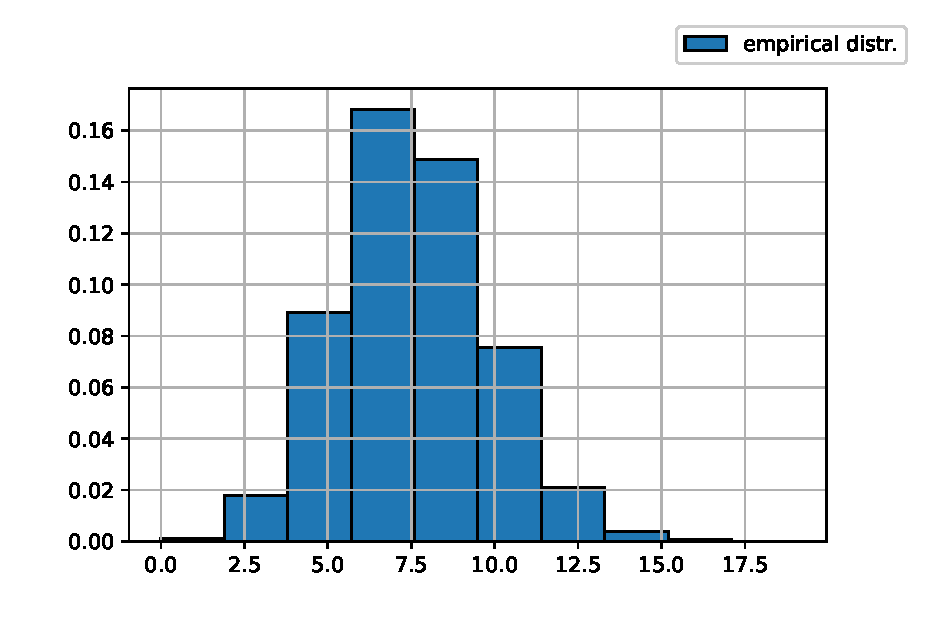
\includegraphics[width=0.7\textwidth]{1_1.eps}\\
		{Рис. 1. Гистограмма биномиального распределения при $p = 1/4, \ n = 30$ }
	\end{center}
	\begin{center}
		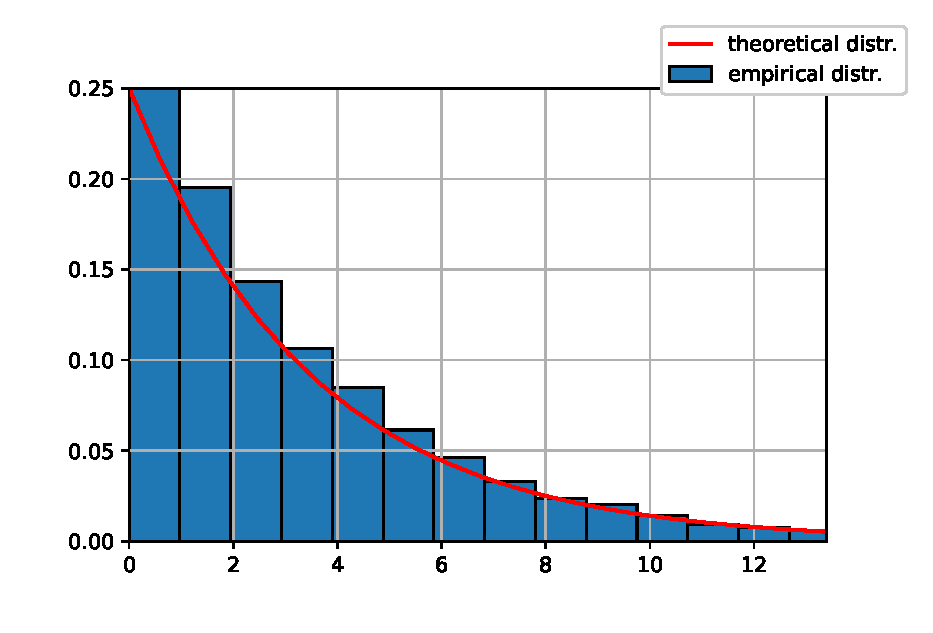
\includegraphics[width=0.7\textwidth]{1_2.eps}\\
		{Рис. 2. Гистограмма геометрического распределения при $p = 1/4$}
	\end{center}
	\begin{center}
		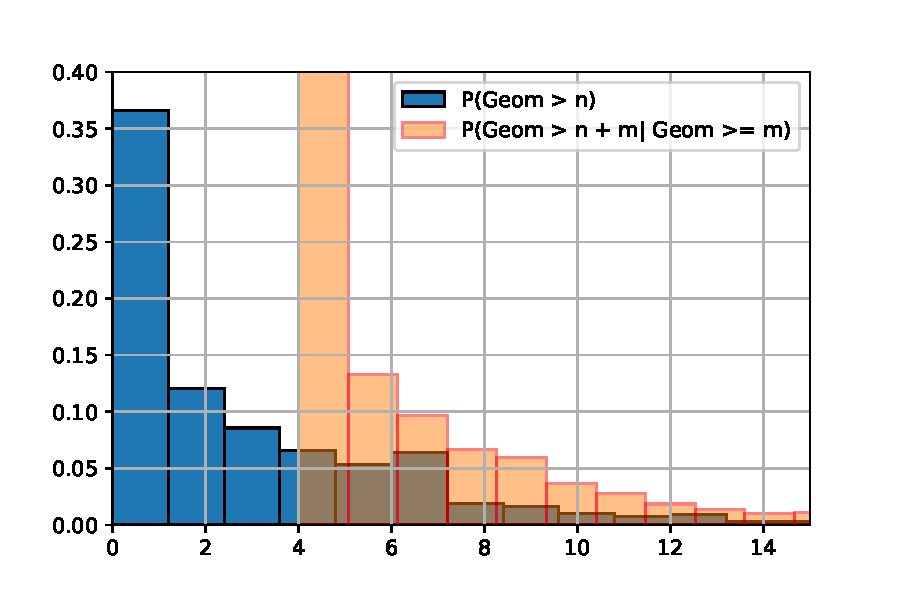
\includegraphics[width=0.7\textwidth]{1_3.pdf}\\
		{Рис. 3. Демонстрация свойства отсутствия памяти при $m = 4, n = 0$}
	\end{center}
	\begin{center}
		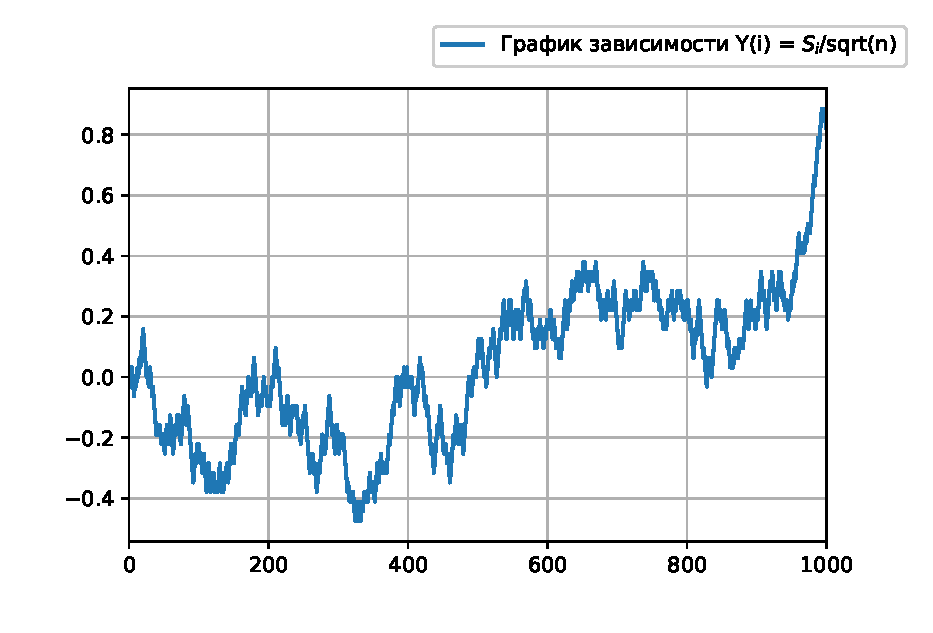
\includegraphics[width=0.7\textwidth]{1_4.eps}\\
		{Рис. 4. Демонстрация игры в орлянку.}
	\end{center}

\newpage
	\section{Задание №2}
	\subsection{Постановка задачи}
	\begin{enumerate}
		\item Построить датчик сингулярного распределения,\ имеющий в качестве функции распределения канторову лестницу.\ С помощью критерия Колмогорова убедиться в корректности работы датчика.
		\item Для канторовых случайных величин проверить свойство симметричности относительно {$\frac{1}{2}$} ({$X$}  и {$1 - X$} распределены одинаково) и самоподобия относительно деления на 3\ (условное распределение Y при условии {$Y \in[0,\frac{1}{3}]$} совпадает с распределением {$\frac{Y}{3}$}) с помощью критерия Смирнова.
		\item Вычислить значение математического ожидания и дисперсии для данного распределения.\ Сравнить теоретические значения с эмпирическими для разного объема выборок.\ Проиллюстрировать сходимость. 
	\end{enumerate}
	
	\subsection{Решение}
	\subsubsection{Сингулярное распределения}
	\begin{opr}
		 Распределение называется сингулярным,\ если оно сосредоточено на континуальном множестве с нулевой мерой Лебега.
	\end{opr}
	\indent Напомним процесс построения канторова множества.\\
	При построении канторова множества {$F$} на отрезке {$[0,1]$} мы выбрасываем из него интервалы {$(\frac{1}{3},\frac{2}{3}),~ (\frac{1}{9},\frac{2}{9}),~ (\frac{7}{9},\frac{8}{9}),\ldots$}\ В итоге получаем замкнутое множество {$F$} (как пересечение замкнутых).\ Оно получается из отрезка {$[0,1]$} выбрасыванием счетного числа интервалов.\\
	Отметим,\ что в канторовом множестве лежат только те точки,\ в записи которых в троичной системе счисления нет единиц.\ Таким образом,\ канторова лестница {$F(X)$} действует на такие точки по правилу:
	$$F(\{a_1,a_2,\ldots,a_n,\ldots\}) = \{b_1,b_2,\ldots,b_n,\ldots\},$$
	где {$a_i$} число в троичной системе счисления, а {$b_i$} число в двоичной системе счисления.\\
	Поэтому будем \textbf{генерировать элементы} данного множества следующим образом:
	$$X = \sum_{k = 1}^{\infty} \frac{2\xi_k}{3^k},~ \text{где}~ \xi_k\sim Ber(0.5).$$
	Суммирование ведется до бесконечности. При построении будем суммировать до некоторого разряда $n \in \mathbb{N}$. \\
	\textbf{Априорная оценка ошибки} равна $\sum_{k = n + 1}^{\infty} \big(\frac{2}{3}\big)^k = 3^{-n} \Rightarrow $ достаточно взять $3^{-n} \leq \varepsilon$ (где $\varepsilon$ --- точность вычислений). Из этого вытекает неравенство $n \geq -\log_3 \varepsilon$ и формула: 
	\[  n = [-\log_3\varepsilon]. \]
	
	\indent Для того,\ чтобы убедиться в корректности работы датчика,\ воспользуемся \textbf{критерием Колмогорова}.\ При проверке согласия по критерию Колмогорова в качестве меры расхождения
	между гипотетическим и истинным распределениями исследуемой случайной величины используется статистика
	$$D_n = \sup\limits_{|x|< \infty} |F^*_n(x) - F(x)|,$$
	представляющая собой точную верхнюю границу абсолютной величины разности
	между гипотетической {$F(x)$} и эмпирической {$F_n^*(x)$},\ полученной по имеющейся выборке,\ функциями распределения.\\
	\[ F_n(x) = \frac{1}{n}\sum_{i = 1}^{n}I_{X_i \leq x}, \  \text{  где  } \ I_{X_i \leq x} = \begin{cases}
	1, & X_i \leq x;\\
	0, & X_i > x.
	\end{cases} \]
	 
	Статистика {$D_n$} вычисляется с помощью формул
	$$D_n^+ = \max\limits_{1\leqslant j \leqslant n} \big\rvert F(x_j) - \frac{j}{n}\big\lvert;$$
	$$D_n^- = \max\limits_{1\leqslant j \leqslant n} \big\rvert F(x_j) - \frac{j - 1}{n}\big\lvert;$$
	$$D_n = \max(D_n^+,D_n^-).$$
	\\
	\indent Обозначим нулевую гипотезу {$ H_{0} $} ,\ как гипотезу о том,\ что выборка подчиняется распределению {$ F(X)$}.\ Тогда по теореме Колмогорова для введённой статистики справедливо:
	
	$$ \forall x>0\colon \lim _{n\to \infty }P({\sqrt {n}}D_{n}\leqslant x)=K(x)=2\sum _{j=1 }^{+\infty }(-1)^{j}e^{-2j^{2}x^{2}}.$$ 
	Т.е. при {$n\longrightarrow \infty $} закон распределения случайной величины {$\sqrt{n}D_n$}\ независимо от вида  распределения случайной величины {$X$} стремится к закону распределения Колмогорова.\\
	Учтём, что критерий имеет правостороннюю критическую область.\ Если статистика {$ {\sqrt {n}}D_{n}$}  превышает процентную точку распределения Колмогорова {$ K_{\alpha }$}  заданного уровня значимости {$ \alpha $} ,\ то нулевая гипотеза {$H_{0}$}  (о соответствии закону {$ F(x)$} отвергается).\ Иначе гипотеза принимается на уровне {$\alpha $} .	
	\begin{table}[h]	
		\begin{center}
			\begin{tabular}[c]{ | c | c | }
				\hline
				Количество запусков & Гипотеза принята \\ \hline
				100 & 95  \\
				1000 & 968   \\
				10000 & 9527  \\
				\hline
				
			\end{tabular}
		\end{center}
		\caption{\label{tab:canonsummary}Критерий Колмогорова}
	\end{table}
	
	
	
	\subsubsection{Свойство симметричности и самоподобия}
	\indent Проверим свойство симметричности относительно {$\frac{1}{2}$} случайных величин {$X~ \text{и}~  1-X$}. Рассмотрим случайную величину  {$1-X$}:
	$$ 1 - X = 1 - \sum_{k = 1}^{\infty}\frac{2\xi_k}{3^k} = \sum_{k = 1}^{\infty}\frac{2}{3^k} - \sum_{k = 1}^{\infty}\frac{2\xi_k}{3^k} =\sum_{k = 1}^{\infty}\frac{2(1 - \xi_k)}{3^k} = \sum_{k = 1}^{\infty}\frac{2\eta_k}{3^k}.$$
	Очевидно,\ что {$\eta_k \sim Bern(0.5)$},\ пэтому {$X~ \text{и}~  1-X$} распределены одинаково.\\
	\indent Проверим свойство самоподобия.\ Рассмотрим условное распределение {$X$} при условии {$X\in [0, 1/3]$}.\ Из построения случайной величины {$X$} видно,\ что  {$X\in [0, 1/3]\Leftrightarrow \xi_1 = 0$}.\ Если {$X\in [0, 1/3]$},\ то
	$$X = \sum_{k = 2}^{\infty}\frac{2\xi_k}{3^k} = \sum_{k = 1}^{\infty}\frac{2\xi_{k+1}}{3^{k+1}} = \frac{1}{3}\sum_{k = 1}^{\infty}\frac{2\xi_k}{3^k} = \frac{1}{3}X.$$
	\indent Для теоретического подтверждения данного факта воспользуемся критерием Смирнова. \\ \textbf{Критерий однородности Смирнова} используется для проверки гипотезы о принадлежности двух независимых выборок одному закону распределения, то есть того,\  что два эмпирических распределения соответствуют одному и тому же закону.\ Статистика критерия Смирнова измеряет различие ме­жду эмпирическими функциями распределения, построенными по выборкам
	$$D_{m,n} = \sup\limits_{|x|<\infty}|G_m(x) - F_n(x)|.$$
	Если гипотеза  справедлива, то при неограниченном увеличении объемов выборок,$$\forall x>0\colon \lim _{m,n\to \infty }P({\sqrt {\frac{nm}{n+m}}}D_{m,n}\leqslant x)=K(x)=2\sum _{j=1 }^{+\infty }(-1)^{j}e^{-2j^{2}x^{2}}$$ т.е. статистика {$\sqrt{\frac{nm}{n+m}}D_{m,n}$} в пределе подчиняется распределению Колмогорова {$K(x)$}.\\
	\indent Если статистика {$ {\sqrt {\frac {nm}{n+m}}}D_{m,\;n}$}  превышает квантиль распределения Колмогорова {$ K_{\alpha }$}  для заданного уровня значимости {$ \alpha $} , то нулевая гипотеза {$ H_{0}$}  (об однородности выборок) отвергается. Иначе гипотеза принимается на уровне {$\alpha$ } .	
	
	\begin{table}[h]	
		\begin{center}
			\begin{tabular}[c]{ | c | c | }
				\hline
				Количество запусков & Гипотеза принята \\ \hline
				100 & 92  \\
				1000 & 913  \\
				10000 & 8945  \\
				\hline
				
			\end{tabular}
		\end{center}
		\caption{\label{tab:canonsummary2}Критерий Смирнова для симметричности }
	\end{table}
	
	\begin{table}[h]	
		\begin{center}
			\begin{tabular}[c]{ | c | c |  }
				\hline
				Количество запусков & Гипотеза принята \\ \hline
				100 & 93  \\
				1000 & 928  \\
				10000 & 8993 \\
				\hline
				
			\end{tabular}
		\end{center}
		\caption{\label{tab:canonsummary3}Критерий Смирнова для самоподобия}
	\end{table}
	\subsubsection{Вычисление математического ожидания и дисперсии}
	\indent Вычислим значение математического ожидания:
	$$\mathbb EX = \mathbb E\sum_{k = 1}^{\infty}\frac{2\xi_k}{3^k} = \sum_{k = 1}^{\infty}\frac{2\mathbb E\xi_k}{3^k} =\sum_{k = 1}^{\infty}\frac{1}{3^k} = \frac{1}{2},\ $$
	где  {$\mathbb E\xi_k = \frac{1}{2} $} --- математическое ожидание случайной величины,\ имеющей распределение Бернулли с параметром  {$p = 0.5$}.  \\
	\indent Вычислим значение дисперсии:
	$$\mathbb DX = \mathbb D\sum_{k=1}^{\infty}\frac{2\xi_k}{3^k} = \{\mathbb D[aX] = a^2\mathbb D[X] -~ \text{свойство}\} = \sum_{k = 1}^{\infty}\frac{4\mathbb D\xi_k}{3^{2k}} = \sum_{k = 1}^{\infty}\frac{1}{3^{2k}} = \frac{1}{8},$$
	где  {$\mathbb D\xi_k = pq = \frac{1}{4} $} --- математическое ожидание случайной величины,\ имеющей распределение Бернулли с параметром  {$p = 0.5~ \text{и}~ q = 1 - p = 0.5$}.
	\subsection{Примеры работы программы}
	\begin{center}
		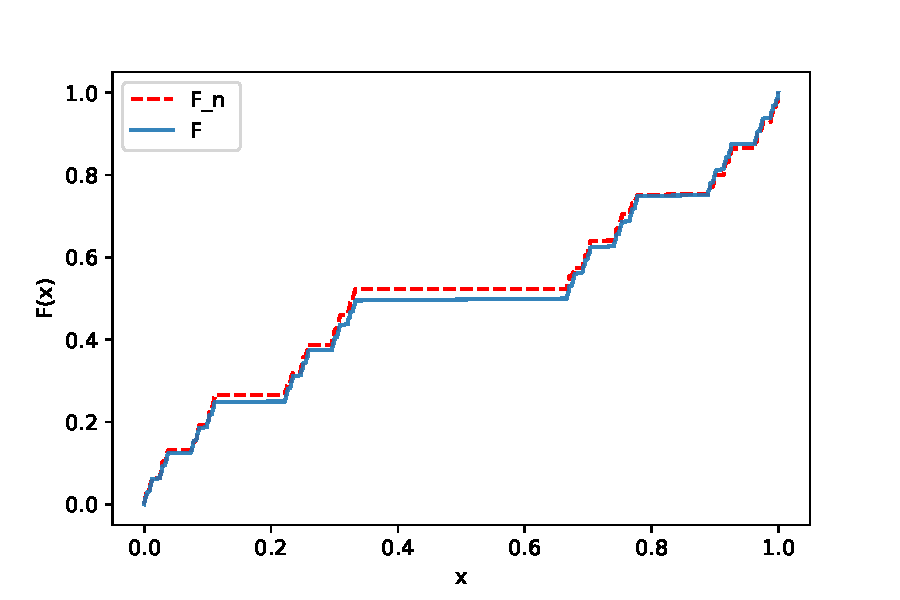
\includegraphics[width=0.7\textwidth]{2_2.pdf}\\
		{Рис. 5. Канторова лестница (теоретическая и эмпирическая) при $n = 1000$.}
	\end{center}
	\begin{center}
		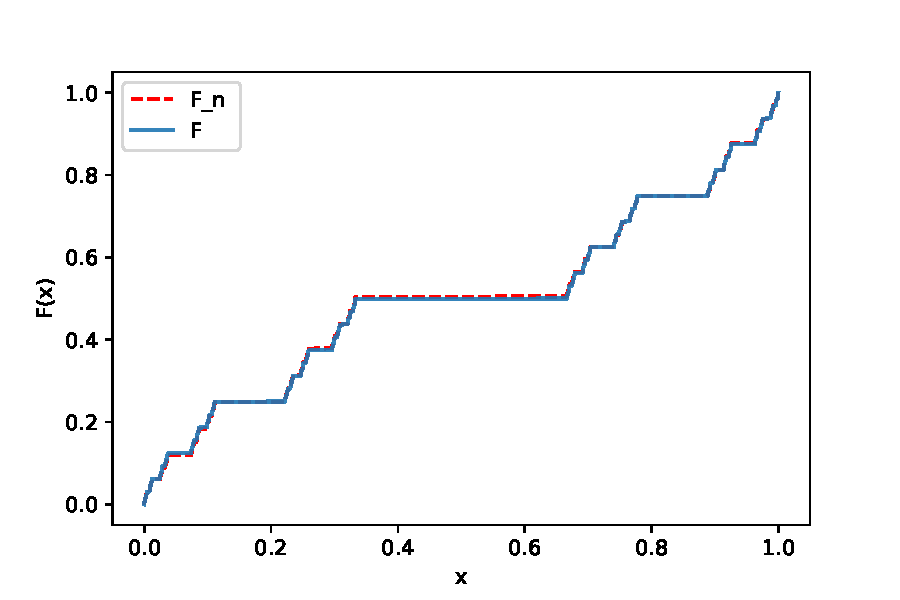
\includegraphics[width=0.7\textwidth]{2_1.pdf}\\
		{Рис. 6. Канторова лестница (теоретическая и эмпирическая) при $n = 10000$. }
	\end{center}
	\begin{center}
		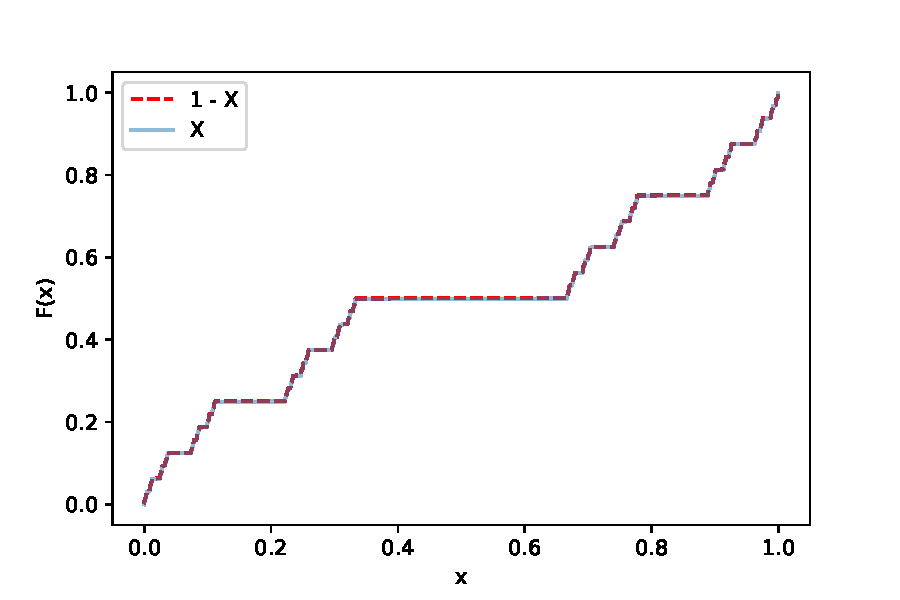
\includegraphics[width=0.7\textwidth]{2_3.pdf}\\
		{Рис. 7. Свойство cимметричности $X \thicksim 1 - X.$  }
	\end{center}
	\begin{center}
		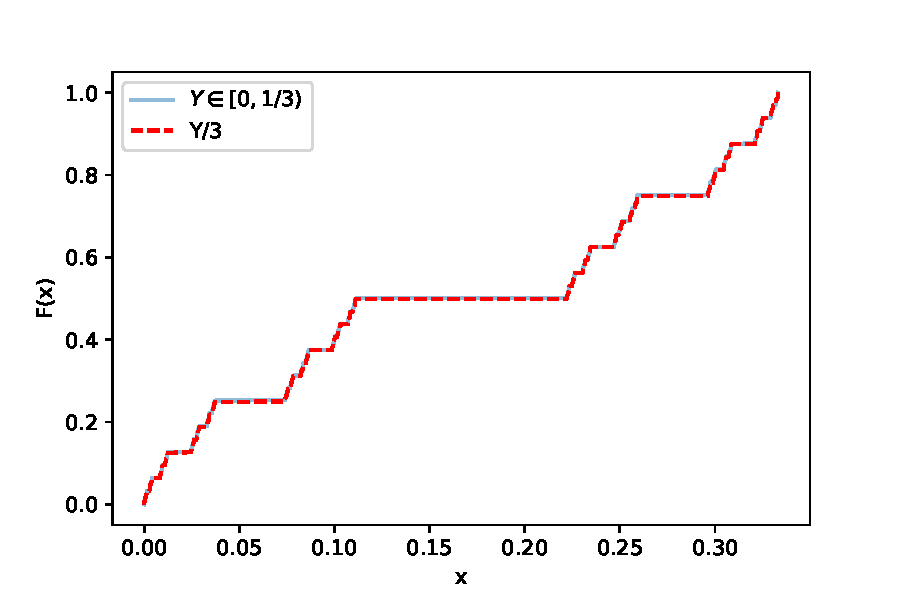
\includegraphics[width=0.7\textwidth]{2_4.pdf}\\
		{Рис. 8. Cвойство самоподобия $Y/3 \thicksim (Y \in [0, 1/3])$. }
	\end{center}
	\begin{center}
		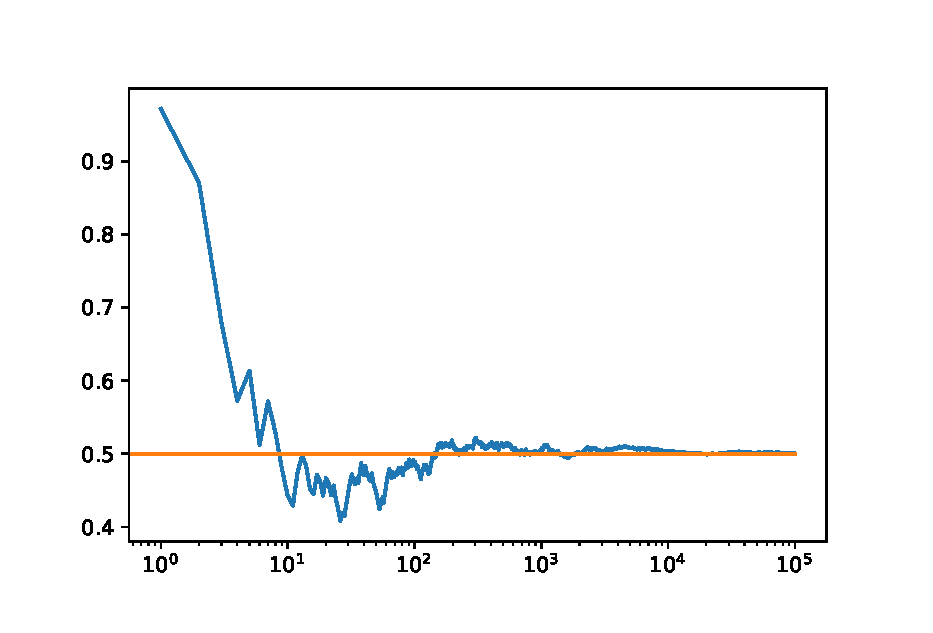
\includegraphics[width=0.7\textwidth]{2_5.eps}\\
		{Рис. 9. Демонстрация сходимости эмпирического математического ожидания к теоретическому.}
	\end{center}
	\begin{center}
		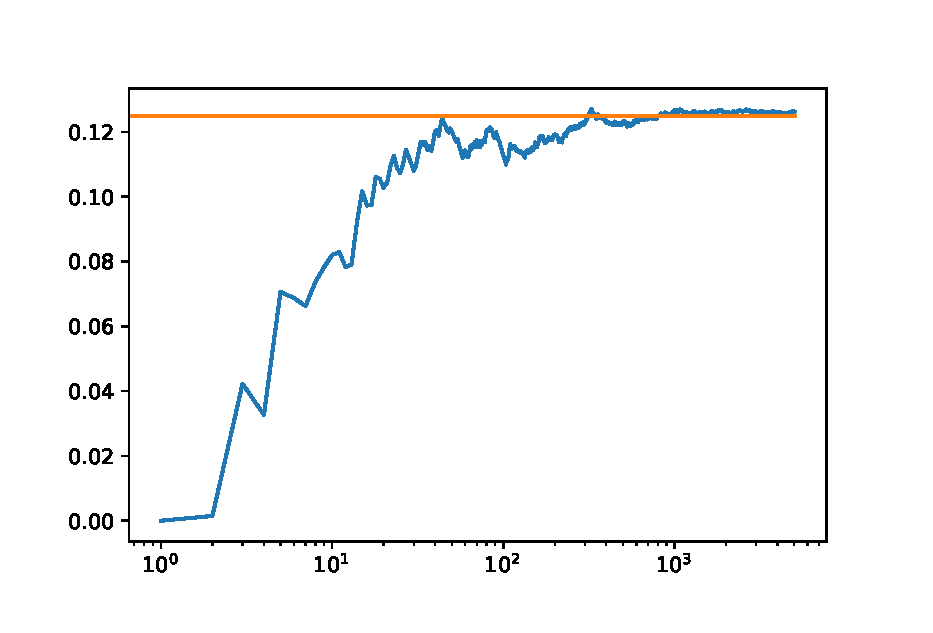
\includegraphics[width=0.7\textwidth]{2_6.eps}\\
		{Рис. 10.  Демонстрация сходимости эмпирической дисперсии к теоретической. }
	\end{center}
	\newpage
	\section{Задание №3}
	\subsection{Постановка задачи}
	\begin{enumerate}
		\item Построить датчик экспоненциального распределения. Проверить для данного распределения свойство отсутствия памяти. Пусть $X_1,X_2,\dots,X_n$--- независимо экспоненциально распределенные с.в. с параметрами $\lambda_1,\lambda_2,\dots, \lambda_n$ соответственно. Найти распределение случайной величины $Y = \min (X_1,X_2,\dots,X_n).$
		\item На основе датчик экспоненциального распределения построить датчик пуассоновского распределения.
		\item Построить датчик пуассоновского распределения как предел биномиального распределения. С помощью критерия хи-квадрат Пирсона убедиться, что получен датчик распределения Пуассона.
		\item Построить датчик стандартного нормального распределения методом моделирования случайных величин парами с переходом в полярные координаты. Проверить при помощи критерия $t$-критерия Стьюдента равенство математических ожиданий, а при помощи критерия Фишера равенство дисперсий.
	\end{enumerate}
	\subsection{Решение}
	\subsubsection{Построение датчика экспоненциального распределения}
	\begin{opr}
		Случайная величина $X$ имеет экспоненциальное распределение с параметром $\lambda > 0,$ если ее функция распределения имеет вид:
		\begin{equation}
		F_X(x) = \begin{cases}
		1- e^{-\lambda x}, & x \leq 0,\\
		0, & x < 0.
		\end{cases}
		\end{equation}
	\end{opr}
	
	\begin{theorem}
		{Пусть на $\mathbb{R}$ определена функция $F(x)$ такая, что:
	\begin{itemize}
		\item $F(x)$ непрерывна,
		\item $F(x)$ монотонно возрастает,
		\item $F(x) \rightarrow 0$ при $x \rightarrow -\infty,$
		\item $F(x) \rightarrow 1$ при $x \rightarrow \infty.$
	\end{itemize}	
	Пусть так же задана с.в. $Y \sim U[0,1].$ Тогда функция $F(x)$ является функцией распределения с.в. $X = F^{-1}(Y).$
}
	\end{theorem} 
	\begin{proof}
		Найдем функцию распределения $X$:
		\[F_X(x) = \mathbb{P}(X < x) = \mathbb{P}(F^{-1}(Y) < x) = P(Y < F(x)) = F(x). \]
	\end{proof}
	Применим эту теорему для моделирования датчика экспоненциального распределения на основе датчика равномерного.
	\[ F_\xi(x) = 1 - e^{-\lambda x} \Rightarrow F_\xi^{-1}(x) = -\frac{1}{\lambda}\ln (1 - x).  \]	
	Таким образом, если $Y \sim U[0,1],$ то:
	\[ X = -\frac{1}{\lambda}\ln (1 - Y) \]
	имеет экспоненциальное распределение с параметром $\lambda.$
	\newline
	Покажем, что экспоненциальное распределение обладает свойством отсутствия памяти. Для этого применим аксиому условной вероятности:
	\[ \mathbb{P}(X \geq s + t| X \geq t) = \frac{\mathbb{P}(X \geq s + t, X \geq t)}{\mathbb{P}(X \geq t)} = \frac{\mathbb{P}(X \geq s + t)}{\mathbb{P}(X \geq t)} = \frac{e^{-\lambda(t + s)}}{e^{-\lambda t}} =  \mathbb{P}(X \geq s). \]
	Это выполнено для $\forall t \neq 0$ и $\forall s.$
	Таким образом получаем:
	\[ \mathbb{P}(X \geq s + t) = \mathbb{P}(X \geq t)\mathbb{P}(X \geq s). \]
	Значит экспоненциальное распределение обладает свойством отсутствия памяти.
	\begin{utv}
		Пусть $X_1,\dots,X_n$ независимые с.в., и $X_i \sim Exp(\lambda_i).$ Тогда $Y = \underset{i = 1,\dots,n}{min}(X_i) \sim Exp(\sum_{i = 1}^{n}\lambda_i).$
		\newline
	\end{utv}	
	\begin{proof}
		Запишем функцию экспоненциального распределения с помощью определения: $\mathbb{P}(X < x) = 1 - e^{-\lambda x} \Rightarrow \mathbb{P}(X > x) = e^{-\lambda x}. $ Тогда $\mathbb{P}(Y = \min (X_1,\dots,X_n) > x) = \mathbb{P}(X_1 > x, \dots, X_n > x) = \{X_1, X_2, \dots, X_n  - \text{независимые с.в.}\} = \prod_{i = 1}^{n}\mathbb{P}(X_i > x) = e^{-\lambda_1 x}\cdot \dots \cdot e^{-\lambda_n x} = e^{-\sum_{i = 1}^{n}\lambda_i x}.$
	\end{proof}
	\subsubsection{Реализация пуассоновского распределения на основе экспоненциального }
	\begin{opr}
		Случайная величина $\xi$ имеет распределение Пуассона с параметром $\lambda,$ если 
		\[ \mathbb{P}(\xi - k) = \frac{\lambda^k}{k!}e^{-\lambda}, \ k = 0,1,2,
		\dots \]
		Обозначение: $X \sim Pois(\lambda).$
	\end{opr}
	\begin{theorem}
		Пусть  $\eta_1,\eta_2, \dots, \eta_n,\dots $--- независимые с.в., такие, что $X_i \sim Exp(\lambda), i = \overline{1,\infty}.$ Если 
		\[\xi = \max\{n: \sum_{i = 1}^{n}\eta_i < 1\},\]
		то случайная величина $\xi \sim Pois(\lambda).$ В случае, если $\eta_1 > 1,$ то полагаем, что $\xi = 0.$
	\end{theorem}
    Доказательство этой теоремы можно найти в [2].
    \newline
    Согласно этому утверждению, можно моделировать нашу с.в. следующим образом: будем генерировать с.в. $\eta_i$ до тех пор, пока их сумма не превзойдет единицу. Тогда с.в. $\xi = i - 1$ будет иметь распределение Пуассона с параметром $\lambda.$
    \subsubsection{Датчик пуассоновского распределения как предел биномиального}
    \begin{theorem}
    	Пусть с.в. $X \sim B(n,p).$ Пусть $np = \lambda = const.$ Тогда при $n \rightarrow \infty:$
    	\[ \mathbb{P}(X = k) = C^k_np^k(1 - p)^{n - k} \rightarrow \frac{\lambda^k}{k!}e^{-\lambda}. \]
    \end{theorem}
	Доказательство этой теоремы можно найти в [2]
	\newline
	Критерий согласия Пирсона(критерий согласия хи-критерий) наиболее часто употребляемый критерий для проверки гипотезы о принадлежности наблюдаемой выборки $x_1,x_2,\dots,x_n$ объемом $n$ некоторому теоретическому закону распределения $F(x,\theta).$
	\newline 
	Будем использовать этот критерий для проверки простой гипотезы:
	\[H_0 : F_n(x) = Pois(x,\lambda). \]
	Исследуемое распределение принимает только целые неотрицательные значения. Обозначим за $n_i$ количество элементов в выборке равных $i$. Теоретическая вероятность выпадения значения $i$ в распределении Пуассона:
	\[ p_i = \frac{\lambda^i}{i!}e^{-\lambda}. \]
	Пусть $k$ --- максимальное значение в выборке. Построим статистику критерия $\chi^2$:
	\[ X_n^2 = n\sum_{i = 1}^{n}\frac{(\frac{n_i}{n} - p_i)^2}{p_i} .\]
	Гипотеза о пуассоновском распределении(с.в.) будет верна, если вычисленное значение статистики не превосходит критического значения $X_{r,\alpha}^2$, где $r = k - 1,\alpha$--- заданный уровень значимости.
	\newline
	Таблица сравнения значений статистики при разных значениях $n$ и $\alpha = 0.95$:
	\newline
	\begin{center}
	\begin{tabular}{|c|c|}
		\hline
		$n$ запусков & Гипотеза принята  \\
		100 & 97  \\
		1000 & 973  \\
		10000 & 9621 \\
		\hline
	\end{tabular}
	\end{center}
	
	\subsubsection{Моделирование датчика стандартного нормального распределения при помощи перехода к полярным координатам}
	\begin{opr}
		Случайная величина $\xi$ имеет нормальное распределение вероятностей  с параметрами $\mu, \sigma^2:\xi \sim \mathcal{N}(\mu,\sigma^2)$($\mu$--- математическое ожидание $\xi$, $\sigma^2$ --- дисперсия $\xi$), если ее плотность распределения задается формулой:
		\[ p_\xi(x)= \frac{1}{\sqrt{2\pi}\sigma}\exp(-\frac{(x - \mu)^2 }{a\sigma^2}), \  -\infty < x < +\infty. \]
	\end{opr}
	\begin{opr}
		Нормальное распределение с параметрами $\mu$ и $\sigma^2 = 1$ называется стандартным нормальным распределением, и ее плотность распределения имеет вид:
		\[ p_\xi(x) = \frac{1}{\sqrt{2\pi}\exp(-\frac{x^2}{2})}, \ -\infty < x < +\infty. \]
	\end{opr}
	Для моделирования стандартного нормального распределения рассмотрим случайную величину $X = \{X_1, X_2\} \sim \mathcal{N}(0,1):$
	\[ \mathbb{P}(X_1 < x_1, X_2 < x_2) = \frac{1}{2\pi}\int_{-\infty}^{x_1}\int_{-\infty}^{x_2}e^{-\frac{\xi^2 + \eta^2}{2}}d\xi d\eta. \]
	Перейдем к полярным координатам:
	\[\xi = \rho \cos \phi, \ \ \eta = \rho \sin \phi. \]
	Учтем Якобиан:
	\[ J = \det \begin{pmatrix}
	\cos \phi & -\rho \sin \phi \\
	\sin \phi & \rho \cos \phi
	\end{pmatrix} = \rho \neq 0. \]
	Тогда 
	\[ \mathbb{P}(X_1 < x_1, X_2 < x_2) = \underset{\rho \cos \phi < x_1 ; \rho \sin \phi < x_2
	}{\int} \frac{1}{2\pi}\frac{1}{2\pi}e^{-\frac{\xi^2 + \eta^2}{2}}d\xi d\eta = \{\omega = \rho^2\} = \underset{\sqrt{\omega} \cos \phi < x_1 ; \sqrt{\omega} \sin \phi < x_2
}{\int} \frac{1}{4\pi}e^{-\frac{\omega}{2}}d\omega d\phi \]	
Подынтегральное выражение является произведением плотностей случайных величин $Y_1 \sim Exp(\frac{1}{2})$ и $Y_2 \sim U[0,2\pi].$ Таким образом, совместное распределение случайных величин $X_1$ и $X_2$ совпадает с совместным распределением:
\[ \{ \sqrt{Y_1}\cos Y_2, \sqrt{Y_1}\sin Y_2 \}, \ Y_1 \sim Exp(\frac{1}{2}), \ Y_2 \sim U[0,2\pi].  \]
Случайные величины $X_1$ и $X_2$ являются независимыми, поскольку их совместное распределение равно произведению их маргинальных распределений:
\[  \mathbb{P}(X_1 < x_2, X_2 < x_2) = \int_{-\infty}^{x_1}\int_{-\infty}^{x_2}\frac{1}{2\pi}e^{-\frac{\xi^2 + \eta^2}{2}}d\xi d\eta = \int_{-\infty}^{x_1}\frac{1}{2\pi} e^{-\frac{\xi^2}{2}d\xi} \int_{-\infty}^{x_2}\frac{1}{2\pi}e^{-\frac{\eta^2}{2}}d\eta. \]
\subsubsection{t-критерий Стьюдента и критерий Фишера}
Проверим равенство математических ожиданий построенных случайных величин $\xi$ и $\eta$, используя t-критерий Стьюдента. Обозначим через $M_1$ и $M_2$ математические ожидания первой и второй выборки соответственно. Рассмотрим разность выборочных средних $\Delta = \overline{\xi} - \overline{\eta}.$
Если нулевая гипотеза о равенстве математических ожиданий выполнена, то математическое ожидание $\mathbb{E}(\Delta) = M_1 - M_2 = 0.$ Зная, что $\mathbb{D}(\xi) = \mathbb{D}(\eta) = 1$, то
\[ \mathbb{D}(\overline{\xi}) = \frac{\mathbb{D}(\sum_{i = 1}^{n}x_i)}{n^2} = \{X_1,\dots, X_n \text{ независимы} \} = \frac{1}{n} = \mathbb{D}(\overline{\eta}), \]
то
\[\mathbb{D}(\Delta) = \frac{2}{n}.\] 
Использую несмещенную оценку дисперсии: $s_1^2 = \frac{\sum_{i = 1}^{n}(\xi_i - \overline{\xi})}{n - 1}$ и $s_2^2 = \frac{\sum_{i = 1}^{n}(\eta_i - \overline{\eta})}{n - 1}$, получаем несмещенную оценку дисперсии разности выборочных средних: $s_\Delta^2 = \frac{s_1^2 + s_2^2}{n}.$ 
\newline 
Значит для проверки нулевой гипотезы t-статистика равна $t = \frac{\overline{\xi} - \overline{\eta}}{\sqrt{s_1^2 + s_2^2}}\sqrt{n}.$
\newline
Если полученное значение статистики $t$ превосходит критическое значение $t_{\alpha,r}$ для заданного уровня значимости $\alpha$, то нулевая гипотеза отвергается.
\newline
Результаты проверки равенства математического ожидания с помощью критерия Стьюдента с $\alpha = 5$\% представлены в следующей таблице:

\begin{center}
\begin{tabular}{|c|c|c|}
\hline
$n$ запусков &Объем выборки & Гипотеза принята \\
100 & 1000 & 98 \\
100 & 10000 & 96 \\
1000& 1000 & 958 \\
1000& 10000 & 944 \\
\hline
\end{tabular}
\end{center}
Теперь опишем критерий Фишера равенства дисперсий. Для ранее определенных величин $s_1^2$ и $s_2^2$ зададим статистику:
\[ F = \frac{s_1^2}{s_2^2}. \]
Проверим равенство дисперсий с помощью критерия Фишера. Если $F < F_{\frac{\alpha}{2}}(n - 1, n -1)$ или $F > F_{1 - \frac{\alpha}{2}}(n-1, n-1),$ то нулевая гипотеза о равенстве дисперсий отвергается, где $F_\alpha(n-1,m-1)$ есть $\alpha$-квантиль распределения Фишера.
\newline
Результаты проверки равенства дисперсий с помощью критерия Фишера с  $\alpha = 5$\% представлены в следующей таблице:
\begin{center}
	\begin{tabular}{|c|c|c|}
		\hline
		$n$ запусков &Объем выборки & Гипотеза принята \\
		100 & 1000 & 95 \\
		100 & 10000 & 96 \\
		1000& 1000 & 948 \\
		1000& 10000 & 946 \\
		\hline
	\end{tabular}
\end{center}


\subsection{Пример работы программы}
\begin{center}
	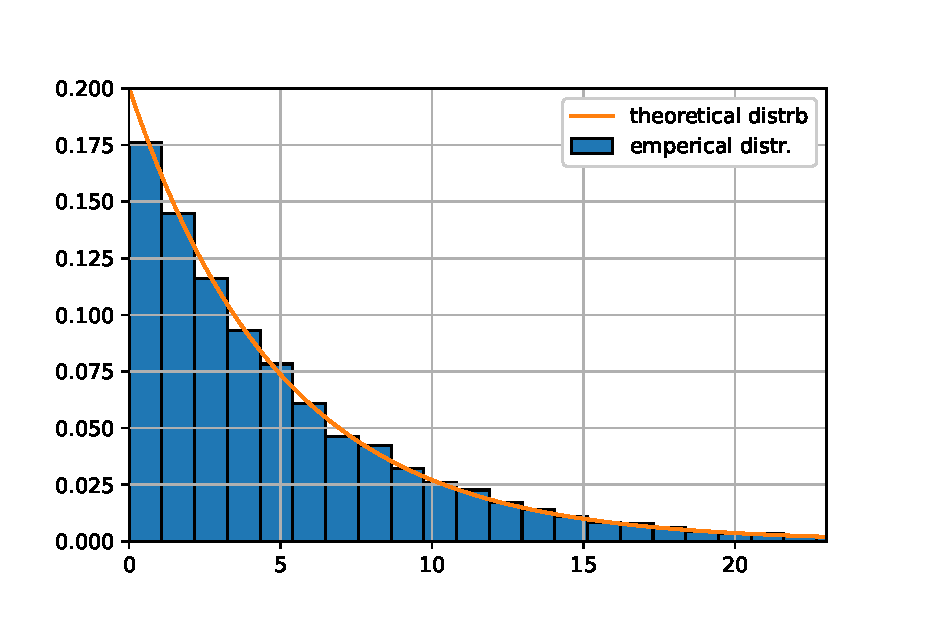
\includegraphics[width=0.7\textwidth]{3_1.eps}\\
	{Рис. 11. Датчик экспоненциального распределения. }
\end{center}
\begin{center}
	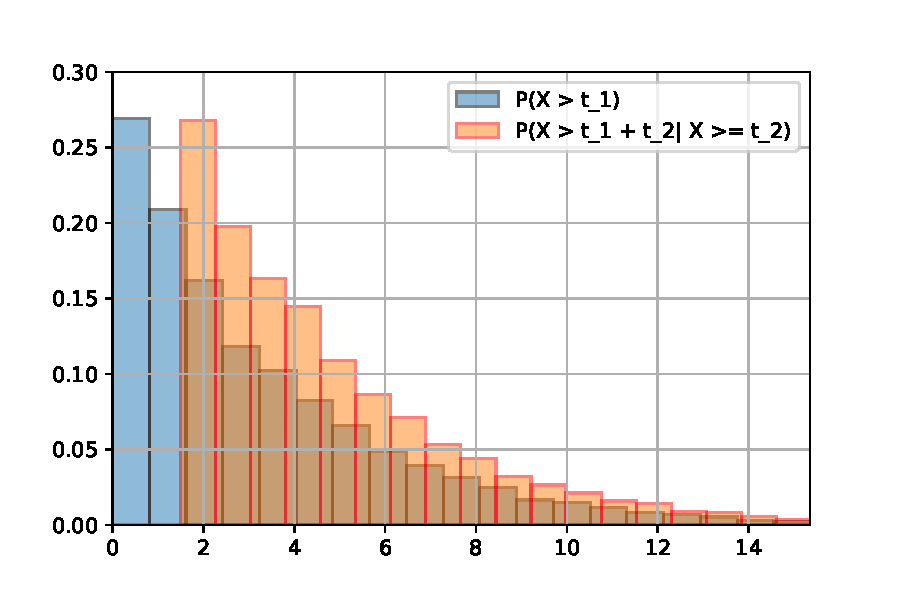
\includegraphics[width=0.7\textwidth]{3_2.pdf}\\
	{Рис. 12. Демонстрация свойства отсутствия памяти геометрического распределения. }
\end{center}
\begin{center}
	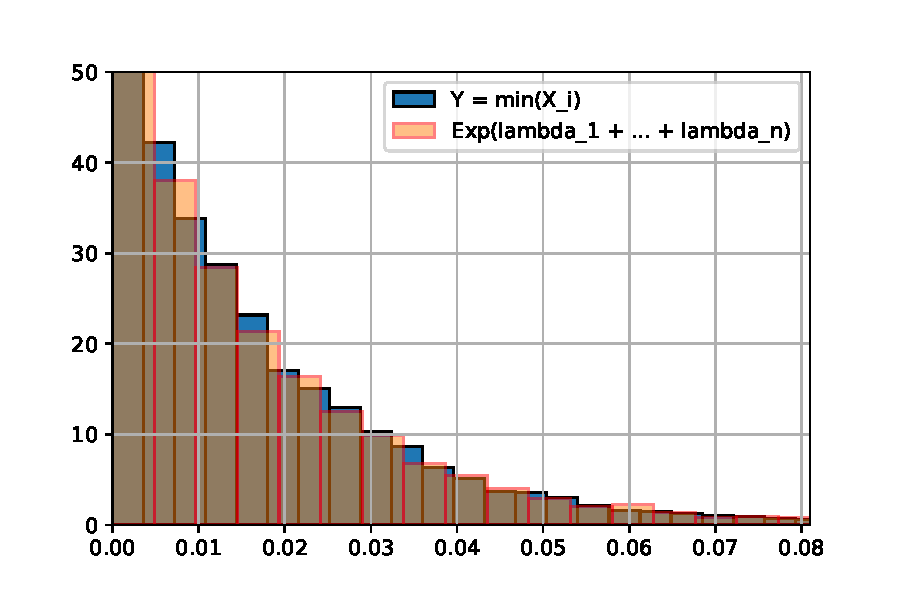
\includegraphics[width=0.7\textwidth]{3_3.pdf}\\
	{Рис. 13.  $Y = \underset{i = 1,\dots,n}{\min}(X_i) \sim Exp\big( \sum_{i = 1}^{n} \lambda_i \big)$. }
\end{center}
\begin{center}
	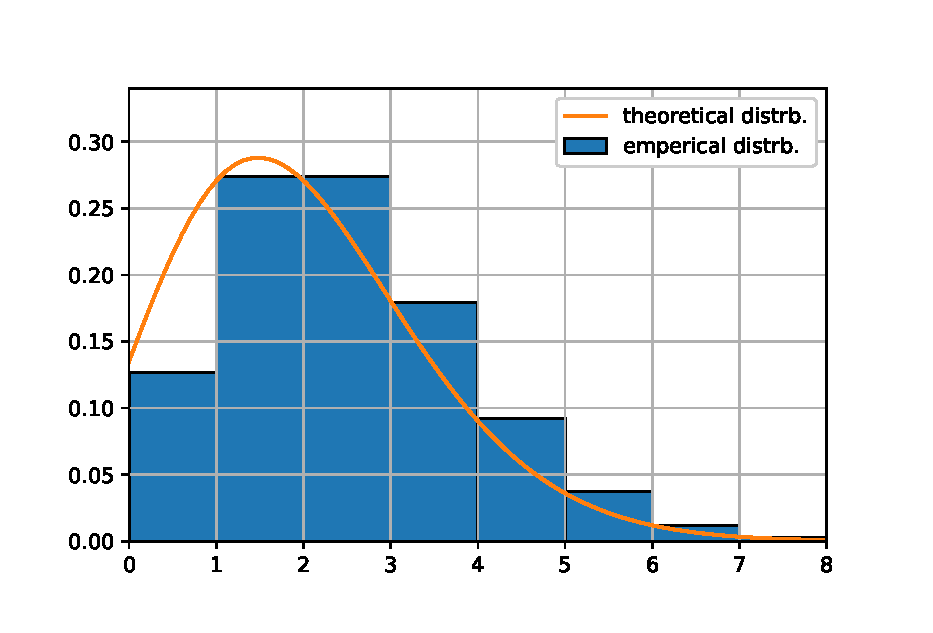
\includegraphics[width=0.7\textwidth]{3_4.eps}\\
	{Рис. 14. Датчик распределения Пуассона на основе экспонециального. }
\end{center}
\begin{center}
	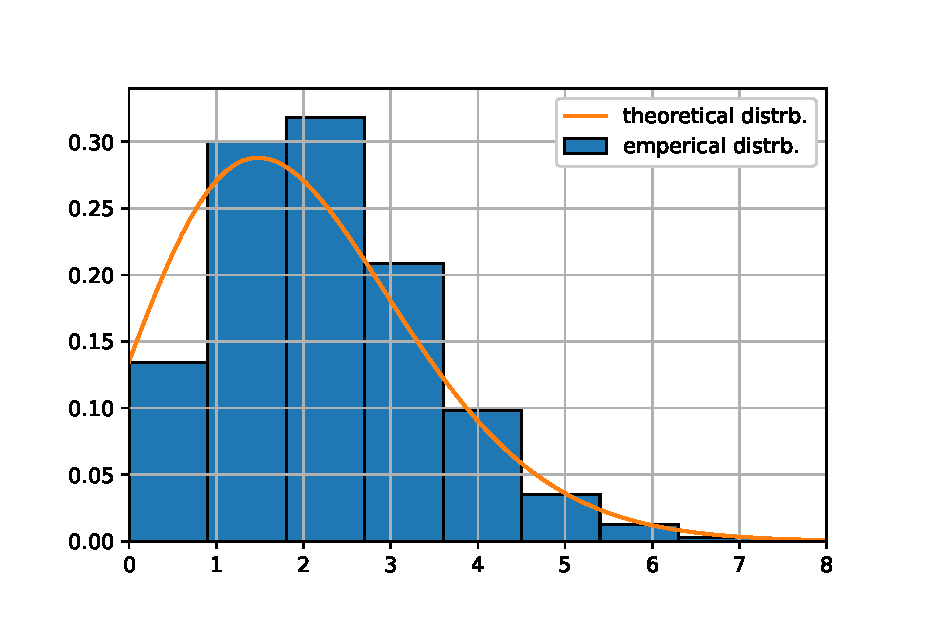
\includegraphics[width=0.7\textwidth]{3_5.eps}\\
	{Рис. 15.  Датчик распределения Пуассона как предел биномиального. }
\end{center}

\newpage

\section{Задание №4}
\subsection{Постановка задачи}
\begin{enumerate}
	\item Построить датчик распределения Коши.
	\item На основе датчика распределения Коши с помощью метода фон Неймана построить датчик стандартного нормального распределения. При помощи функции normal probability plot убедится в корректности построенного датчика и обосновать наблюдаемую зависимость.
	\item Сравнить скорость моделирования стандартного нормального распределения в задания 3 и 4.
\end{enumerate}
\subsection{Решение}
\subsubsection{Датчик распределения Коши}
\begin{opr}
	Случайная величина $X$ имеет распределение Коши с параметрами $a$ и $b$, если ее функция распределения имеет вид:
	\[ F_X(x) = \frac{1}{\pi}\arctan\bigg(\frac{x - a}{b}\bigg) + \frac{1}{2} \]
	Плотность распределения Коши имеет вид:
	\[ p_X(x) = \frac{1}{\pi} \frac{b}{(x - a)^2 + b^2}. \]
\end{opr}
Функция распределения с.в. $F_X(x)$ удовлетворяет условиям теоремы 1 из задания 3. Обратная функция для данного распределения равно $F^{-1}_X(y) = a + b\tan(\pi(y - \frac{1}{2}))$. Значит, в качестве датчика распределения Коши можно построить датчик случайной величины $X = F^{-1}_X(Y),$ где $Y \sim U[0,1].$
\subsubsection{Метод фон Неймана}
Метод фон Неймана заключается в моделировании нормального распределения путем мажорирования плотностью распределения Коши с параметрами $a$ и $b$. Для достижения наилучшей оценки, будем подбирать параметры $a$ и $b$.\\
Плотность стандартного нормального распределения $p_1(x)$ и плотность распределения Коши $p_2(x)$ выглядят следующим образом:
\[ p_1(x) = \frac{1}{\sqrt{2\pi}}e^{-\frac{x^2}{2}}, \]
\[p_2(x) = \frac{1}{\pi}\frac{b}{(x- a)^2 + b^2}. \]
При моделировании будем следовать алгоритму:
\begin{enumerate}
	\item возьмем некоторое число $k > 0$, такое, что $p_1(x) \leq kp_2(x), \ \forall x \in \mathbb{R},$ 
	\item рассмотрим значение случайно величины $x = X,$ где $X \sim Cauchy(a,b),$
	\item сгенерируем случайную величину $y = Y(x) \sim Bern\big(\frac{p_1(x)}{kp_2(x)}\big), $
	\item если $y = 1,$ то $x$--- значение из распределения $p_1(x)$, иначе --- переходим к пункту 2 алгоритма и продолжаем моделирование.
\end{enumerate}
Чем ближе отношение $\frac{p_1(x)}{kp_2(x)}$ к единице, тем быстрее работает данный алгоритм, поэтому в качестве $k$ возьмем $k^* = \underset{a,b}{\min} \ \underset{x}{\max}\frac{p_1(x)}{p_2(x)}$. Рассмотрим отношение: 
\[ \frac{p_1(x)}{p_2(x)} = \frac{\sqrt{\pi}}{\sqrt{2}b}((x - a)^2 + b^2)e^{-\frac{x^2}{2}}. \]
Пусть $a = 0$. Рассмотрим вспомогательную функцию:
\[ g(x) = (x^2 + b^2)e^{-\frac{x^2}{2}}. \]
Найдем максимум этой функции:
\[ g^{'}(x) = e^{-\frac{x^2}{2}}x(2 - b^2 - x^2) = 0 \]
Корнями данного уравнения будут: $x = 0 $ при $|b| > \sqrt{2}$ и $x = \pm \sqrt{2 - b^2}$ при $0 < |b| \leq \sqrt{2}.$
Тогда получим:
\[ k^* = \min \bigg\{\underset{|b| > \sqrt{2}}{\min}\sqrt{\frac{\pi}{2}}b, \underset{0 < |b| < \sqrt{2}}{\min} \frac{\sqrt{2\pi}}{b}e^{\frac{b^2}{2} - 1} \bigg\}. \]
Так как $k > 0$, то и $b > 0$. Найдем максимум вспомогательной функции $h(b) = \frac{e^{\frac{b^2}{2} - 1}}{b}$:
\[ h^{'}(b) = \frac{1 - b^2}{b^2}e^{\frac{b^2}{2} - 1}.\]
Поскольку $b > 0$, то получим единственную точку экстремума $b = 1.$\\
Значит получим оптимальную точку при $a^* = 0, b^* = 1:$
\[ k^* = \min \bigg\{ \sqrt{\pi},\sqrt{\frac{2\pi}{e}} \bigg\} = \sqrt{\frac{2\pi}{e}}. \]
Докажем, что $a = 0$ --- оптимальное значение параметра.


\begin{eqnarray*}
k^* = \underset{a.b}{\min} \ \underset{x}{\max}\bigg(\frac{\sqrt{\pi}}{\sqrt{2}b}e^{-\frac{x^2}{2}}((x - a)^2 + b^2)\bigg) = \underset{a}{\min} \bigg\{ \underset{b > \sqrt{2}}{\min} \  \frac{p_1(x)}{p_2(x)}\bigg|_{x = 0}, \underset{0 < b \leq \sqrt{2}}{\min} \ \frac{p_1(x)}{p_2(x)}\bigg|_{x = \pm \sqrt{2 - b^2}} \bigg\} > \\ 
>  \underset{a}{\min} \bigg\{ \underset{b > \sqrt{2}}{\min}   \frac{\sqrt{\pi}}{\sqrt{2}b}(a^2 + b^2), \underset{0 < b \leq \sqrt{2}}{\min}\big( \sqrt{2 - b^2} + |a| \big) \bigg\}
\end{eqnarray*}
Минимум выражения достигается при $a = 0.$\\
Иллюстрация работы построенного датчика, которая использует функцию normal probability plot, представлена в пункте с демонстраций работы программы. График функции распределения стандартной нормальной с.в. представляют прямую. На оси абсцисс откладываются точки выборки, на оси ординат --- квантили стандартного нормального распределения.\\
Возьмем случайную величину $\xi \sim \mathcal{N}(\mu,\sigma^2).$ Тогда функция распределения:
\[F_\xi(x) = \frac{1}{\sqrt{2\pi\sigma^2}}\int_{-\infty}^{x}\exp(-\frac{(t - \mu)^2}{2\sigma^2})dt .\]
Сделаем замену переменной $s = \frac{t - \mu}{\sigma}.$ Тогда:
\[ F_\xi(x) = \frac{1}{\sqrt{2\pi}}\int_{-\infty}^{\frac{x - \mu}{\sigma}}\exp(-\frac{s^2}{2})ds = F(\frac{x - \mu}{\sigma}) \]
где $F(x)$ --- функция стандартного нормального распределения.\\
Таким образом, квантили различных распределений связаны между собой линейно, что означает, что любую нормальную с.в. $\xi \sim \mathcal{N}(\mu, \sigma^2)$ можно представить в виде $\xi = \sigma\eta + \mu,$ где $\eta \sim \mathcal{N}(0,1),$ а функция normal probability plot будет прямой со сдвигом в $\mu$ и с коэффициентом наклона $\sigma$, то есть корню из дисперсии.
\subsubsection{Сравнение скоростей работы моделирования с.в.}
\begin{table}[h]
	\begin{center}
		\begin{tabular}{|c|c|c|}
			\hline
			$n$ случайных величин & метод фон Неймана & метод перехода к полярным координатам  \\
			100 & 0.0327 & 0.00045 \\
			1000 & 0.2459 & 0.00145 \\
			10000 & 2.1496  & 0.002608 \\
			\hline
		\end{tabular}
		
	\end{center}
	\caption{Время работы методов при разных количествах с.в.}
\end{table}


\subsection{Примеры работы программы}
\begin{center}
	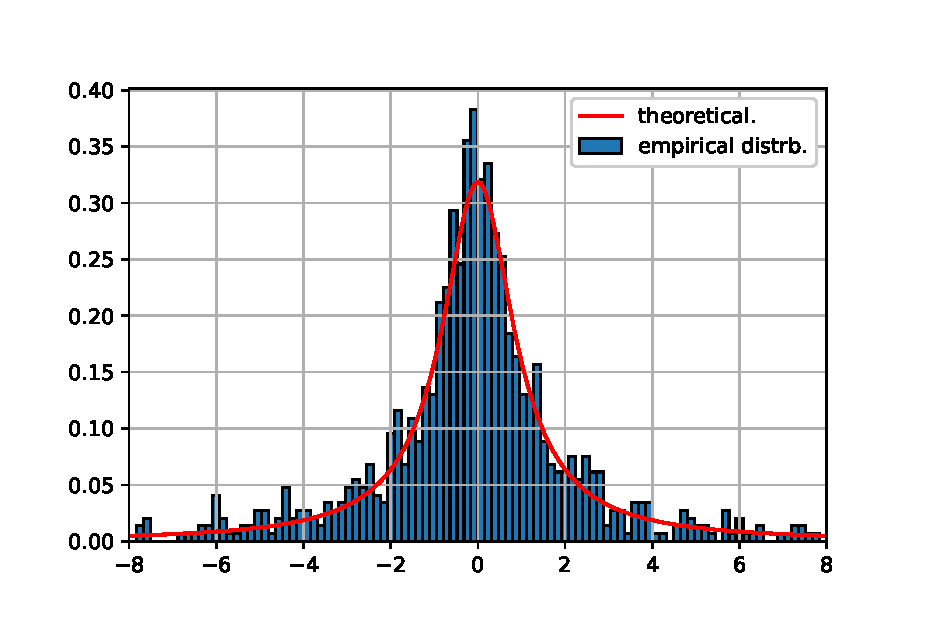
\includegraphics[width=0.7\textwidth]{4_1.eps}\\
	{Рис. 16. Гистограмма распределения Коши. }
\end{center}
\begin{center}
	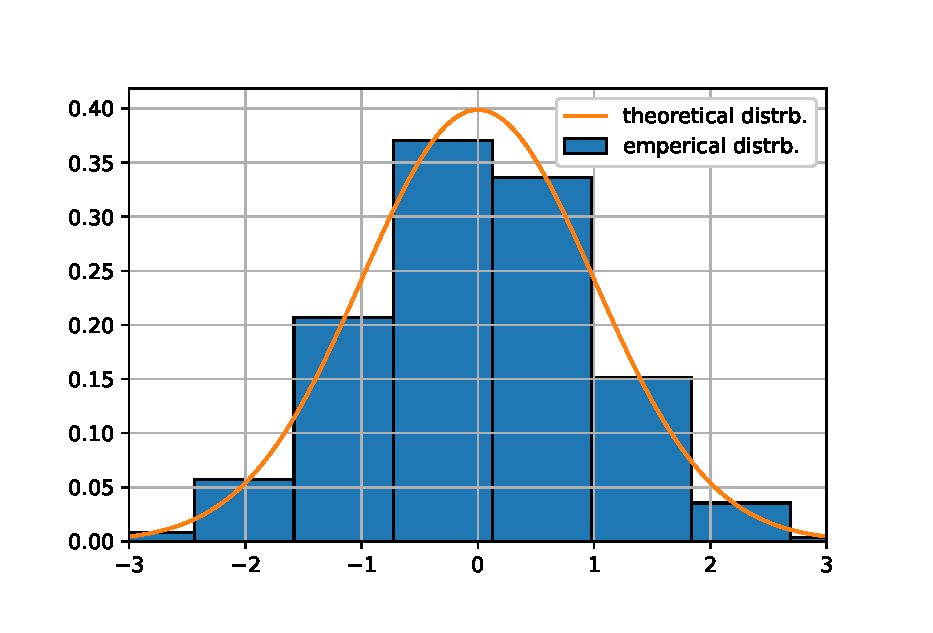
\includegraphics[width=0.7\textwidth]{4_2.eps}\\
	{Рис. 17. Гистограмма нормального распределения, построенная с помощью метода фон Неймана, где $\mu = 0, \sigma = 1, n = 100000$. }
\end{center}
\begin{center}
	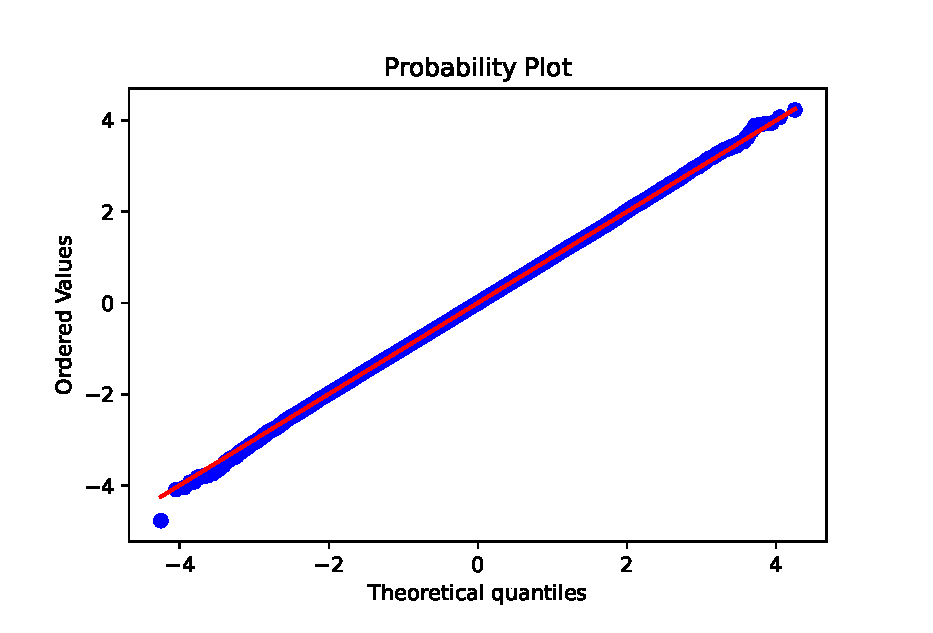
\includegraphics[width=0.7\textwidth]{4_3.eps}\\
	{Рис. 18. Демонстрация работы функции normal probability plot при $\mu = 0, \sigma = 1, n = 100000$. }
\end{center}
\newpage
\section{Задание 5}
\subsection{Постановка задачи}
\begin{enumerate}
	\item Пусть $X_i \sim N(\mu. \sigma^2)$. Убедиться эмпирически в справедливости ЗБЧ и ЦПТ, т.е. исследовать поведение суммы $S_n$ и эмпирического распределения величины
	\[ \sqrt{n}\bigg( \frac{S_n}{n} - \mu \bigg) \]
	\item Считая $\mu$ и $\sigma^2$ неизвестными, для пункта 1 построить доверительные интервалы для среднего и дисперсии.
	\item  Пусть $X_i \sim K(a,b)$ имеет распределение Коши со сдвигом $a$ и масштабом $b$. Проверить эмпирически, как ведут себя суммы $S_n/n$. Результат работы объяснить а также найти закон распределения данных сумм. 
\end{enumerate} 

\subsection{Решение}
\subsubsection{Закон больших чисел(ЗБЧ) и центральная предельная теорема(ЦПТ) для нормального распределения}
Пусть $X_i \sim N(\mu, \sigma^2).$ Исследуем поведение суммы $\frac{S_n}{n}$ и эмпирического распределения величины
\[  \sqrt{n}\bigg( \frac{S_n}{n} - \mu \bigg). \] 
\begin{theorem}
	\textbf{(ЗБЧ)} Пусть $X_1,X_2,\dots$--- независимые одинаково распределенные с.в., $\mathbb{E}X_i = \mu, \forall i \in \mathbb{N}, |\mu| < \infty, S_n = X_1 + \dots + X_n.$ Тогда
	\[ \forall \varepsilon > 0 \ \mathbb{P}\bigg( \bigg|\frac{S_n}{n} - \mu\bigg| \geq \varepsilon \bigg) \underset{n \rightarrow \infty}{\longrightarrow} 0. \]
\end{theorem}
\begin{theorem}
	\textbf{(ЦПТ)} Пусть $X_1,X_2,\dots$--- независимые одинаково распределенные с.в., $0 < \mathbb{E}X_i^2 < \infty, \forall i \in \mathbb{N}, S_n = X_1 + \dots + X_n.$ Тогда
	\[ \mathbb{P}\bigg(\frac{S_n - \mathbb{E}S_n}{\sqrt{\mathbb{D}S_n}}\bigg) \underset{n \rightarrow \infty}{\longrightarrow} \Phi(x), \]
	где $\Phi(x)$--- функция стандартного нормального распределения:
	\[ \Phi(x) = \frac{1}{\sqrt{2\pi}}\int_{-\infty}^{x}e^{-\frac{u^2}{2}}du. \]  
\end{theorem}
Доказательство данных теорем представлено в [2].
\subsubsection{Доверительные интервалы для среднего и дисперсии}
Рассмотрим случайную величину $X \sim N(\mu,\sigma^2).$ Пусть $x_1,x_2,\dots,x_n$--- ее реализации.\\
Введем обозначения:
\[ \textbf{Выборочное среднее --- } \overline{x} = \frac{1}{n}\sum_{i = 1}^{n}x_i ;\]
\[ \textbf{Выборочная дисперсия --- } s^2 = \frac{1}{n - 1}\sum_{i = 1}^{n}(x_i - \overline{x})^2.\]
Для параметров строятся следующие точные доверительные интервалы:
\begin{enumerate}
	\item Для неизвестного среднего $\mu$ при неизвестной дисперсии $\sigma^2$:
	\[ \overline{x} - \frac{s}{\sqrt{n}}t_\gamma < \mu < \overline{x} + \frac{s}{\sqrt{n}}t_\gamma, \]
	где $t_\gamma$--- критическая точка распределения Стьюдента (распределение Коши с параметрами $a = 0, b = 1$) с $n - 1$ степенями свободы и уровнем значимости $\alpha = 1 - \gamma$
	\item Для неизвестной дисперсии:
	\[ \frac{(n - 1)s^2}{\chi^2_{\frac{\alpha}{2},n-1}} < \sigma^2 < \frac{(n - 1)s^2}{\chi^2_{1 - \frac{\alpha}{2},n-1}},  \]
	где $\chi^2_{n-1}$--- критические точки $\chi^2$--- распределения с $n - 1$ степенями свободы и соответствующими уровнями значимости $\alpha = 1 - \gamma.$
\end{enumerate}	
\subsubsection{ЗБЧ для распределения Коши}

Пусть $X_i\sim C(a,b),\ \forall i\in\mathbb{N}$. Рассмотрим график:
\begin{center}
	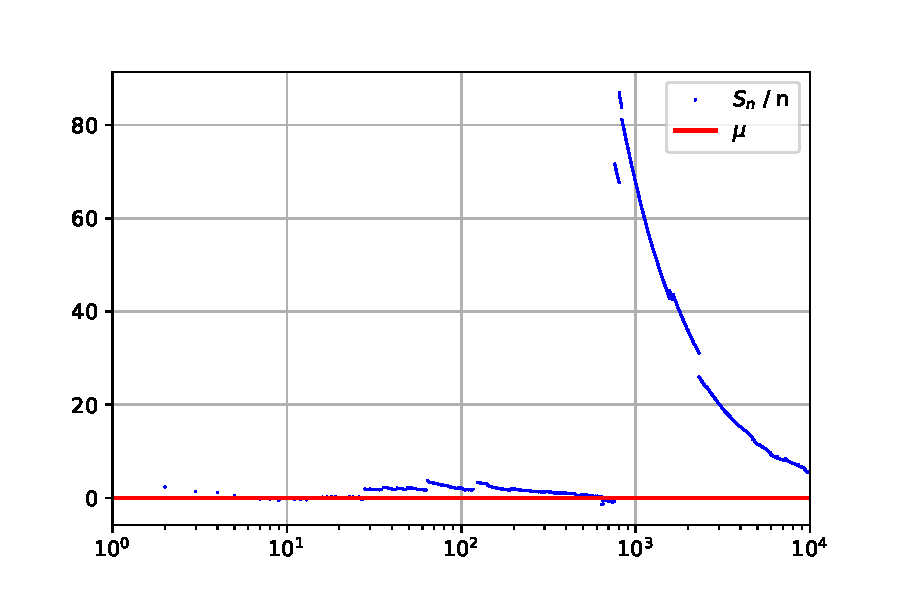
\includegraphics[width=0.7\textwidth]{5_1.pdf}\\
	{Рис. 19. Закон больших чисел для распределения Коши ($S_n / n$) при $\mu = 0, \sigma = 1$ }
\end{center}
На рисунке видно, что $\dfrac{S_n}{n}$ не имеет предела, то есть закон больших чисел для распределения Коши не выполняется. Заметим, что это можно объяснить тем, что мы не можем найти математического ожидания от нашей случайной величины, то есть, мы нарушает одно из условий теоремы о ЗБЧ. Докажем, что математическое ожидание случайной величины $X\sim C(a,b)$ не является конечным:
$$
\mathbb{E} X=\dfrac{1}{\pi}\int\limits_{-\infty}^{\infty} \dfrac{bx}{(x-a)^2+b^2}dx=\left.\dfrac{b}{2\pi}\ln((x-a)^2+b^2)\right|_{-\infty}^{\infty}=\infty-\infty.
$$
Следовательно, эмпирический результат соответствует теории.

\begin{utv}
	Если случайные величины \( \xi_1,\ldots,\xi_n \) независимы и имеют все одно и то же распределение Коши, то среднее арифметическое \( \overline{\xi}=\dfrac{1}{n}\sum\limits_{i=1}^n\xi_i \) имеет то же распределение, что и каждое \( \xi_j \).
\end{utv}
\begin{proof}
	Докажем это утверждение с помощью характеристической функции распределения Коши:
	\[ \varphi(t) = \mathbb{E}e^{it\xi} = \frac{1}{\pi}\int_{}^{}\frac{be^{itx}}{(x - a)^2 + b^2}dx = \frac{e^{ita}}{\pi}\int_{}^{}\frac{e^{itbx}}{x^2 + 1} = e^{ita - |t|b}. \]
	Следовательно характеристическая функция $\frac{S_n}{n}$ имеет вид
	\[ \varphi_{\frac{S_n}{n}}(t) = \bigg(\varphi\bigg(\frac{t}{n}\bigg)\bigg)^n = \varphi(t), \]
	$\Rightarrow$ $\frac{S_n}{n} \sim Cauchy(a,b)$.
\end{proof}
	




\subsection{Примеры работы программы}
\begin{center}
	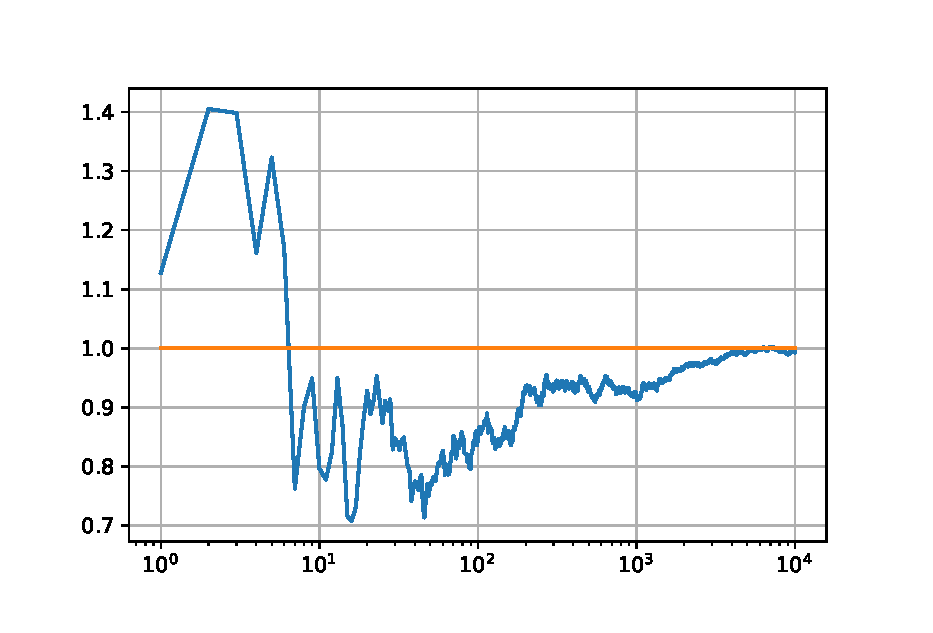
\includegraphics[width=0.7\textwidth]{5_2.eps}\\
	{Рис. 20. Закон больших чисел для нормального распределения при $\mu = 0, sigma = 1$. }
\end{center}
\begin{center}
	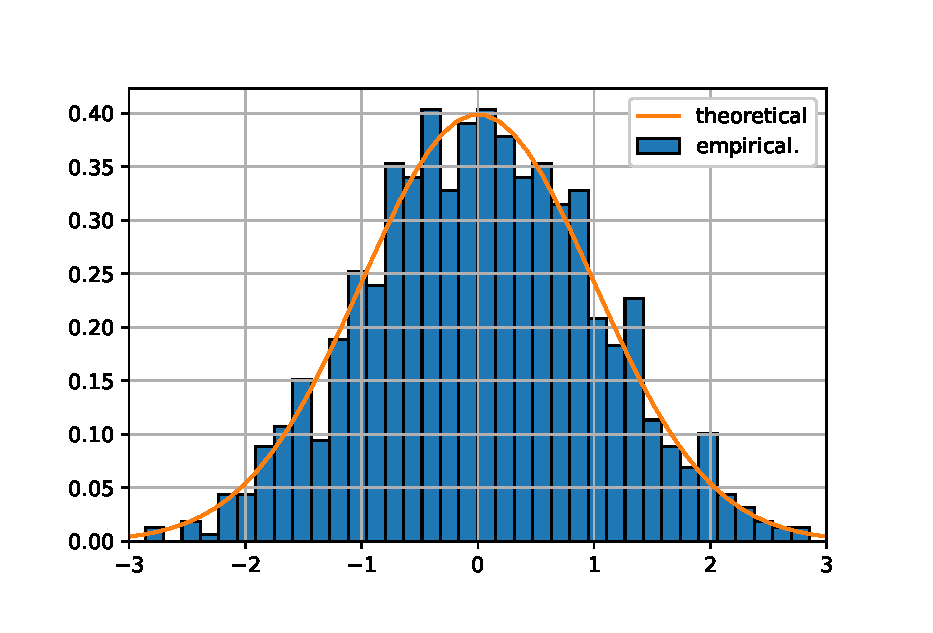
\includegraphics[width=0.7\textwidth]{5_3.eps}\\
	{Рис. 21. Центральная предельная теорема для нормального распределения при $\mu = 0, \sigma = 1$. }
\end{center}
\begin{center}
	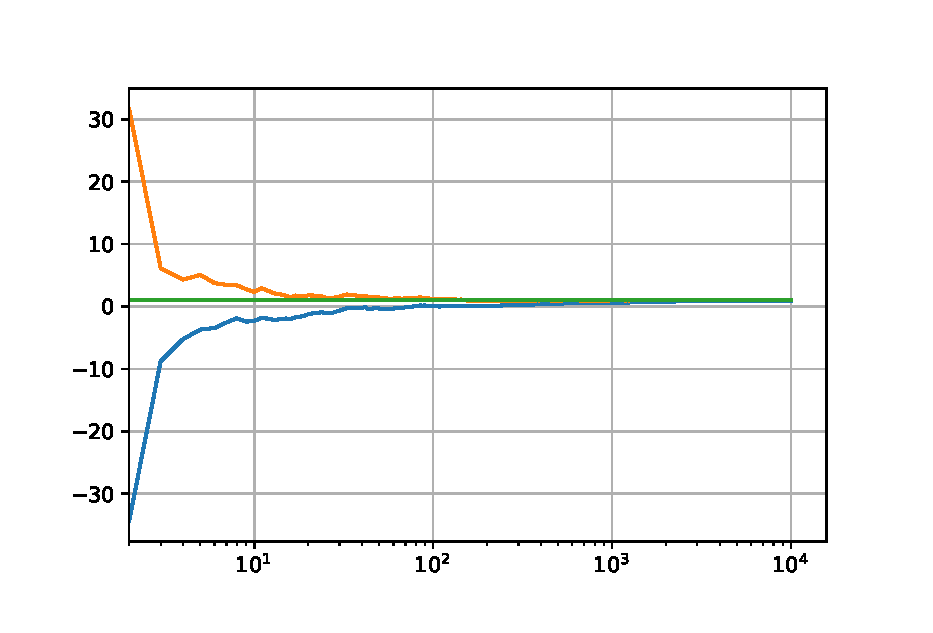
\includegraphics[width=0.7\textwidth]{5_4.eps}\\
	{Рис. 22. Демонстрация доверительного интервала для математического ожидания при $\mu = 1, \sigma = 3$. }
\end{center}
\begin{center}
	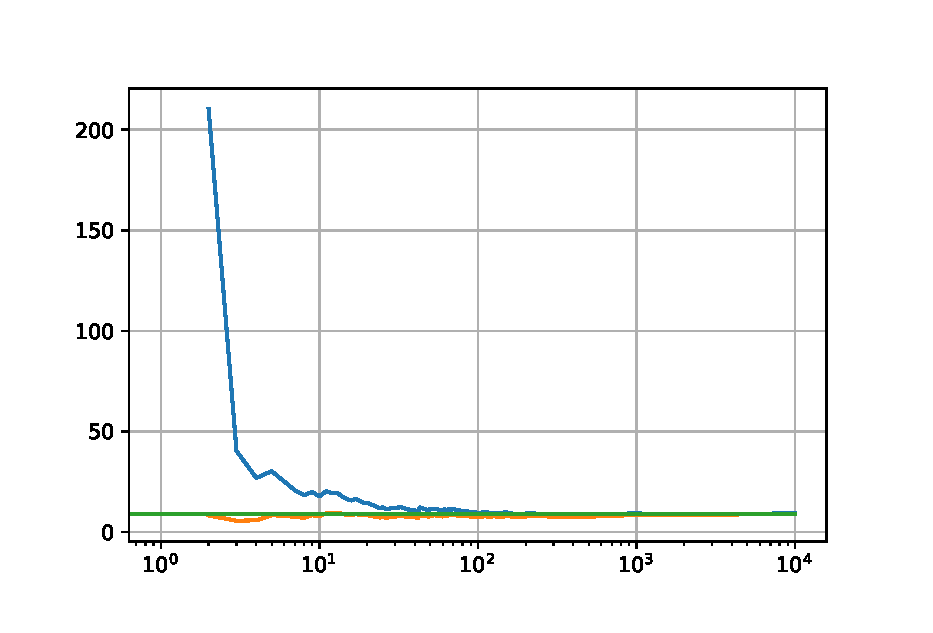
\includegraphics[width=0.7\textwidth]{5_5.eps}\\
	{Рис. 23. Демонстрация доверительного интервала для дисперсии при $\mu = 1, \sigma = 3$. }
\end{center}

\newpage
\section{Задание 6}
\subsection{Постановка задачи}
\begin{enumerate}
	\item Посчитать интеграл		
	\[ \int\limits_{-\infty}^\infty \int\limits_{-\infty}^\infty\dots  \int\limits_{-\infty}^\infty \frac{e^{-\bigg(x_1^2 + \dots + x_{10}^2 + \frac{1}{2^7\cdot x_1^2 \cdot \dots \cdot x_{10}^2}\bigg)}}{x_1^2 \cdot \dots \cdot x_{10}^2}dx_1\dots dx_{10} \] 
	--- методом Монте-Карло 
	\newline
	--- методом квадратур, сводя задачу к вычислению собственного интеграла Римана
	\item Для каждого случая оценить точность вычислений
\end{enumerate}
\subsection{Решение}
\subsubsection{Метод Монте-Карло}
Перепишем интеграл 
\[ \int\limits_{-\infty}^\infty \int\limits_{-\infty}^\infty\dots  \int\limits_{-\infty}^\infty \frac{e^{-\bigg(x_1^2 + \dots + x_{10}^2 + \frac{1}{2^7\cdot x_1^2 \cdot \dots \cdot x_{10}^2}\bigg)}}{x_1^2 \cdot \dots \cdot x_{10}^2}dx_1\dots dx_{10} \] 
в виде
\[ \int\limits_{-\infty}^\infty \int\limits_{-\infty}^\infty\dots  \int\limits_{-\infty}^\infty f(x_1,\dots,x_{10})g(x_1,\dots,x_{10}), \]
где 
\[ f(x) = \sqrt{\pi^{10}}\cdot \frac{e^{-\frac{1}{2^7\cdot x_1^2 \cdot \dots \cdot x_{10}^2}}}{x_1^2 \cdot \dots \cdot x_{10}^2}, g(x) = \frac{1}{\sqrt{\pi^{10}}}\cdot e^{-(x_1^2 + \dots + x_{10}^2)}. \]
Заметим, что $g(x)$ является совместной плотностью распределения набора независимых случайных величин, имеющих нормальное распределение с параметрами 0 и $\frac{1}{2}$:
\[ x = (x_1,\dots,x_{10}), \ x_i \sim N(0,\frac{1}{2}). \]
Тогда интеграл можно записать в виде:
\[ I = \mathbb{E}f(x_1,\dots,x_{10}), \ x_i \sim N(0,\frac{1}{2}). \]
Рассмотрим выборку
\[x^i = (x^i_1,\dots, x^i_{10}), \ x_k^i \sim N(0,\frac{1}{2}), \ k = \overline{1,10}, \ i = \overline{1,n}. \]
Согласно ЗБЧ выборочное среднее будет стремится к математическому ожиданию, то есть:
\[ \overline{f} = \frac{S_n}{n} = \frac{1}{n} \sum_{i = 1}^{n}f(x^i) \underset{n \rightarrow \infty}{\longrightarrow} I. \]
Оценим погрешность метода Монте-Карло с помощью центральной предельной теоремы:
\begin{eqnarray*}
\mathbb{P}\bigg(\bigg|\frac{S_n}{n} - I \bigg| < \varepsilon \bigg) = \mathbb{P}\bigg(\bigg|\frac{S_n - nI}{n} \bigg| < \varepsilon\bigg) = \mathbb{P}\bigg(\bigg|\frac{S_n - nI}{\sigma \sqrt{n}}\bigg| < \frac{\sqrt{n}}{\sigma}\varepsilon \bigg) = \\ 
=\mathbb{P}\bigg( -\frac{\sqrt{n}}{\sigma}\varepsilon  < \frac{S_n - nI}{\sigma\sqrt{n}} < \frac{\sqrt{n}}{\sigma}\varepsilon\bigg) = \Phi_0\bigg(\frac{\sqrt{n}}{\sigma}\varepsilon\bigg) - \Phi_0\bigg(-\frac{\sqrt{n}}{\sigma}\varepsilon\bigg) = \\
= \Phi_0(\frac{\sqrt{n}}{\sigma}\varepsilon) - \bigg(1 - \Phi_0\bigg(\frac{\sqrt{n}}{\sigma}\varepsilon\bigg) \bigg) = 1 - 2\Phi_0\bigg(\frac{\sqrt{n}}{\sigma}\varepsilon\bigg) = 1 - 2\Phi_0\bigg(x_p\bigg) = \alpha,
\end{eqnarray*}
где
\begin{itemize}
	\item [\textbullet]$\Phi_0(x)$ --- функция Лапласа или функция ошибок:
	\[ \Phi(x) = \frac{1}{\sqrt{2\pi}}\int_{-\infty}^{x}e^{-\frac{t^2}{2}}dt,\]
	\item [\textbullet] $x_p = \frac{\sqrt{n}}{\sigma}\varepsilon$--- квантиль уровня $p$. То есть решение уравнения:
	\[ \Phi_0(x_p) = p,  \]
	\item [\textbullet] $\alpha$ --- уровень доверия. 
\end{itemize}
Погрешность $\varepsilon$ для соответствующего уровня доверия $\alpha = 1 - 2\Phi_0(x_p)$ связана с $x_p$ соотношением:
\[ \varepsilon = \frac{\sigma x_p}{\sqrt{n}}.\]
Значение $\sigma > 0$ используем как значение выборочной дисперсии:
\[ \sigma = \frac{1}{n}\sum_{i = 1}^{n}f^2(x_i) - \bigg( \frac{1}{n}\sum_{i = 1}^{n}f(x_i)\bigg)^2. \]
В качестве значения уровня доверия возьмем $\alpha = 0.99$.
\[  \mathbb{P}\bigg( \bigg|\frac{S_n}{n} - I \bigg| < \varepsilon\bigg) = \alpha = 0.99.\]
Продемонстрируем зависимость вычисления значения интеграла и полученной погрешность при разном количестве испытаний:
\begin{center}
	\begin{tabular}{|c|c|c|c|}
		\hline
		Количество итераций &Результат & Погрешность & Время работы \\
		$10^2$ & 104.0312 & 256.1975 & 0.0042\\
		$10^3$ & 177.1406 & 105.7845 & 0.06 \\
		$10^4$ & 106.8784 & 25.8910 & 0.3467 \\
		$10^5$ & 119.2904 & 9.1013  & 3.3645 \\
		$10^6$ & 126.8015 & 2.9583& 25.7833\\
		$10^7$ & 124.8890 & 0.9287& 229.4606\\
		$10^8$ & 124.8630 & 0.2935& 2205.1636\\
		\hline
	\end{tabular}
\end{center}
\subsubsection{Метод квадратур}
Сведем задачу к вычислению собственного интеграла Римана. Для этого сделаем следующую замену переменных:
\[ x_i = \tan\bigg(\frac{\pi}{2}t_i \bigg), \ t_i \in [0,1]. \]
Таким образом по методу прямоугольников исходный интеграл приблизится значением:
\[ I = \bigg(\frac{\pi}{2} \bigg)^{10} \int_{-1}^{1}\dots\int_{-1}^{1}\frac{\exp\Bigg[- \Bigg( \sum_{k = 1}^{10}\tan\bigg(\frac{\pi}{2}t_k\bigg)^2 + \frac{1}{2^7 \cdot \prod_{k = 1}^{10}\tan\bigg(\frac{\pi}{2}t_k\bigg)^2 }\Bigg)\Bigg]}{\prod_{k = 1}^{10}\tan\bigg(\frac{\pi}{2}t_k\bigg)^2 \cdot \prod_{k = 1}^{10}\cos\bigg(\frac{\pi}{2}t_k \bigg)^2}dt_1\dots d_{10}. \]
Проведем равномерное разбиение отрезка $[0,1]$ на $N$ частей:
\[ -1 = t_0 < t_1 < \dots < t_N = 1, \ t_i = -1 + i \cdot \frac{1 - (-1)}{N} = i \cdot \frac{2}{N} - 1. \]
Обозначим через $f(t_1,\dots,t_{10})$ подынтегральную функцию интеграла $I$. Будем использовать метод средних прямоугольник. Для этого нужно выбрать середины отрезков:
\[ y_i = \frac{t_i + t_{i -1}}{2}, \ i = \overline{1, N}. \]
Тогда интеграл можно приближенно посчитать следующим образом:
\[ I_N + \bigg( \frac{\pi}{N}\bigg)^{10} \sum_{i_1 = 1}^{N}\dots \sum_{i_{10} = 1}^{N}f(y_{i_1},\dots,y_{i_{10}}). \]
Оценка погрешности метода прямоугольников на равномерной сетке имеет вид:
\[ \varepsilon = \frac{h^2}{24}(b - a)\sum_{i,j = 1}^{10}\max \bigg|f^{''}_{x_i,x_j} \bigg| = \frac{1}{6N^2}\sum_{i,j = 1}^{10} \max \bigg|f^{''}_{x_i,x_j} \bigg|. \]
Приведем таблицу зависимости результата от количества точек разбиения отрезка:
\begin{center}
	\begin{tabular}{|c|c|c|}
		\hline
		$N$ &Результат  & Время работы \\
		3 & 1.2988 & 2.7317 \\
		4 & 272.7333 & 39.5054  \\
		5 & 183.4885 & 312.2850  \\
		
		\hline
	\end{tabular}
\end{center}
\newpage
\section{Задание 7}
\subsection{Постановка задачи}
\begin{enumerate}
	\item Методом случайного поиска найти минимальное значение функции $f$ на множестве $A = \{x_1,x_2,:x_1^2 + x_2^2 \leq 1 \}$, т.е. $y = \underset{x \in A}{\min}f(x)$, где
	\[ f(x) = x_1^3\sin\bigg(\frac{1}{x_1}\bigg) + 10x_1x_2^4\cos\bigg(\frac{1}{x_2} \bigg) \]
	при $x_1 \neq 0$ и $x_2 \neq =$, функция доопределяется по непрерывности при $x_1 = 0$ или $x_2 = 0$. 
	\item Методом имитации отжига найти минимальное значение функции Розенброка $g$ в пространстве $\mathbb{R}^2$, где 
	\[ g(x) = (x_1 - 1)^2 + 100(x_2 - x_1^2)^2\]
	\item Оценить точность. Сравнить результаты со стандартными методами оптимизации.
\end{enumerate}

\subsection{Решение}
\subsubsection{Метод случайного поиска}
Возьмем единичный круг и сгенерируем на нем набор равномерно распределенных по нему точек. Найдем минимальное значение функции $f$.\\
Совместная плотность равномерного распределения случайных величин $x_1,x_2$ на единичном круге равна:
\[ f_{x_1,x_2} = \begin{cases}
 \frac{1}{\pi}, & x_1^2 + x_2^2 \leq 1,\\
 0, & \text{в противном случае.}
\end{cases} \]
В полярных координатах:
\[  \begin{cases}
x_1 = r\cos\phi, & 0 \leq r \leq 1,\\
x_2 = r\sin\phi, & 0 \leq \phi \leq 2\pi
\end{cases} \]
Таким образом получим:
\begin{equation}
\mathbb{P}((x_1,x_2)\in A) = \underset{x_1^2 + x_2^2 \leq 1}{\iint}\frac{1}{\pi}dx_1dx_2 = \frac{1}{\pi} \int_{0}^{1}rdr\int_{0}^{2\pi}d\phi = \int_{0}^{1}dr^2 \int_{0}^{2\pi}\frac{1}{2\pi}d\phi.
\end{equation}
Сделаем замену:
\[ q = r^2, r = \sqrt{q}, q\in [0,1]. \]
Тогда выражение (2) примет вид:
\[\mathbb{P}((x_1,x_2) \in A) = \int_{0}^{1}dq\int_{0}^{2\pi}\frac{1}{2\pi}d\phi. \]
Следовательно, $x_1$ и $x_2$ выражаются в виде:
\[ \begin{cases}
x_1 = \sqrt{q}\cos\phi, & q \sim U[0,1],\\
x_2 = \sqrt{q}\sin\phi, & \phi \sim U[0,2\pi].
\end{cases} \]
\subsubsection{Метод имитации отжига}
Алгоритм основывается на воссоздании физического процесса, который происходит при кристаллизации вещества, в том числе пр отжиге металлов. Предполагается, что атомы уже выстроились в кристаллическую решетку, но ещё допустимы переходы отдельных атомов из одной ячейку в другую. Предполагается, что процесс протекает при постепенно понижающейся температуре. Переход атома из одной ячейки в другую происходит с некоторой вероятностью, причем вероятность понижается с понижением температуры. Устойчивая кристаллическая решетка соответствует минимуму энергии атомов, поэтому атом либо переходит в состояние с меньшим уровнем энергии, либо остается на месте.\\
При помощи моделирования такого процесса ищется такая точка или множество точек, на котором достигается минимум некоторой числовой функции $F(\overline{x})$, где $\overline{x} = (x_1,\dots,x_m) \in X.$ Решение ищется последовательным вычислением точек $\overline{x_0},\overline{x_1},\dots,$ пространства $X$; каждая точка, начиная с $\overline{x_1},$ <<претендует>> на то, чтобы лучше предыдущих приближать решение. Алгоритм принимает точку $\overline{x_0}$ как исходные данные. На каждом шаге алгоритм вычисляет новую точку и понижает исходно положительную величину (<<температуру>>). Алгоритм останавливается при определенных условия, а именно --- нулевая температура.\\
Точка $\overline{x_{i+1}}$ по алгоритму получается на основе текущей точке $\overline{x_i}$ следующим образом. К точке $\overline{x_i}$ применяется оператор $A$, который случайным образом модифицирует собственную точку, в результате чего получается новая точка $\overline{x^*}$. Точка $\overline{x^*}$ становится точкой $\overline{x_{i+1}}$ с вероятностью $P(\overline{x^*},\overline{x_{i+1}})$, которая вычисляется в соответствии с распределением Гиббса:
\[ P(\overline{x^*} \rightarrow \overline{x_{i+1}}|\overline{x_i}) = \begin{cases}
1, & F(\overline{x^*}) - F(\overline{x_i}) < 0,\\
\exp\bigg(-\frac{F(\overline{x^*}) - F(\overline{x_i})}{T_i}\bigg), & F(\overline{x^*}) - F(\overline{x_i}) \geq 0.
\end{cases}\]
Здесь $T_i > 0$ --- элементы произвольной убывающей, сходящейся к нулю положительной последовательности, которая задает аналог падающей температуры в кристалле. Скорость убывания и закон убывания могут быть заданы по желанию создателя алгоритма.\\
Результаты работы программы по поиску минимума значения функции Розенброка методом отжига приведены в следующей таблице($x^0 = (0,0), \ n = 100$):
\begin{center}
	\begin{tabular}{|c|c|}
		\hline
		Кол-во запусков программы & Минимальное значение \\
		100 & -1.288345  \\
		100 & -1.288486   \\
		10000 & -1.288488 \\
		
		\hline
	\end{tabular}
\end{center}
\subsubsection{Оценка точности вычислений}
Пусть $x = (x_1,x_2)$ --- фактическая точка минимума, $\overset{\sim}{x} =  (\overset{\sim}{x}_1,\overset{\sim}{x}_2)$ --- точка минимума, полученная методом случайного поиска. Оценим $|x - \overset{\sim}{x}|.$ Рассмотрим график исследуемой функции.\\
Исследуемая функция четная по $x_1,x_2,$ имеет несколько точек минимума, которые не являются граничными. Тогда
\[ |x - \overset{\sim}{x}| \leq \varepsilon = \sqrt{\frac{p}{n}}. \]
Оценим $|f(x) - f(\overset{\sim}{x})|$ через $|x - \overset{\sim}{x}|$.\\
Поскольку $f$ --- непрерывна, то $f$ --- липшицева, следовательно:
\[|f(a) - f(b)| \leq ||\nabla f ||_\infty |a-b| = \underset{a,b\in A}{essup}|\nabla f||a-b| = \underset{a,b \in A}{\max}|\nabla f||a-b|, \forall a,b \in A. \]
Оценим $\underset{x_1,x_2 \in A}{\max}|\nabla f|:$
\[ \bigg|\frac{\partial f}{\partial x_1}\bigg| = \bigg|3x_1^2\sin\bigg(\frac{1}{x_1}\bigg) - x_1\cos\bigg(\frac{1}{x_1}\bigg) + 10x_2^4\cos\bigg(\frac{1}{x_2}\bigg) \bigg| \leq 3x_1^2 + |x_1| + 10x_2^4 \leq \sqrt{10} + 10, \]
\[ \bigg|\frac{\partial f}{\partial x_2}\bigg| = \bigg|40x_1x_2^3\cos\bigg(\frac{1}{x_2}\bigg) - 10x_1x_2^2 \sin\bigg(\frac{1}{x_2}\bigg) \bigg| \leq 10\sqrt{17}. \]
Следовательно, $|\nabla f| = \sqrt{\big(\frac{\partial f}{\partial x_1}\big) + \big(\frac{\partial f}{\partial x_2} \big)} = \sqrt{(\sqrt{10} + 10)^2 + (10\sqrt{17})^2}\leq 34.26.$
Окончательная оценка точности вычислений:
\[ |f(x) - f(\overset{\sim}{x}) \leq 34.26 \sqrt{\frac{p}{n}}. \]

\newpage

\section{Задание 8}
\subsection{Постановка задачи}
Применить метод Монте-Карло к решению первой краевой задачи для двумерного уравнения Лапласа в единичном круге:
\begin{equation}
\begin{cases}
\Delta u = 0,(x,y) \in D \\
u|_{\delta D} = f(x,y) \\
u \in C^2(D), f \in C(\delta D)\\
D = \{x,y: x^2 + y^2 \leq 1 \}
\end{cases}
\end{equation}

Для функции $f(x,y) = x^2 - y^2$ найти аналитическое решение и сравнять с полученным по методу Монте-Карло.
 
\subsection{Решение}
Для приближенного решения задачи выберем на плоскости достаточно мелкую квадратную сетку с шагом $h$. Координаты узлов пусть будут $x_i = ih,y_j = jh$, а значения $u(x_i.y_j),f(x_i,y_j)$ обозначим $u_{i,j}f_{i,j}$.
\begin{opr}
	Узел $(x_i,y_j)$ называют внутренним, если он и все четыре соседних с ним узла $(x_{i-1},y_j),(x_{i+1},y_j),(x_i,y_{j-1}),(x_i,y_{j+1})$ принадлежит $\overline{D}$, в противном случае узел называют граничным.
\end{opr}
Обозначим через $D_h$ --- множество внутренних точек, а через $\delta D_h$ --- множество граничных точек. \\
Во внутреннем  узле $(x_i,y_j)$ уравнение Лапласа $u_{xx} + u_{yy} = 0$ заменим разностным уравнением:
\[ \frac{u_{i+1} - 2u_{i,j} + u_{i-1,j}}{h^2} + \frac{u_{i,j+1} -2u_{i,j} + u_{i,j-1}}{h^2} = 0, \]
которое можно переписать в виде
\[u_{i,j} = \frac{1}{4}(u_{i-1,j} + u_{i+1,j} + u_{i,j-1} + u_{i,j+1}).  \]
В граничном узле положим
\[u_{i,j} = f_{i,j}. \]
Представим себе частицу $M$, которая совершает равномерное случайное блуждание по узлам сетки. А именно, находясь во внутреннем узле $(x_i,y_j)$ сетки, эта частица за один переход с одной и той же вероятностью равной 1/4 может переместиться в один из четырех соседних узлов $(x_{i-1},y_j),(x_{i+1},y_j),(x_i,y_{j-1}),(x_i,y_{j+1})$ причем каждый такой единичный переход совершенно случаен и не зависит от положения частицы её прошлой истории. Будем считать, что блуждание заканчивается как только попадает в граничную точку.\\
Пусть $P(i,j,p,q)$ --- вероятность того, что траектория частицы, вышедшей из узла $(x_i,y_j)$, закончится в граничном узле $(x_q,y_q)$. Так как блуждание точки неизбежно заканчивается на границе в первой же точке ее выхода на границу, то 
\[ \sum_{(x_q,y_q) \in \delta D_h}^{}P(i,j,p,q) = 1, \]
причем если $(p',q'),(p,q)\in \delta D_h$, то 
\[ P(p',q',p,q) = \begin{cases}
1, & (p' - p)^2 + (q' - q)^2 =0,\\
0, & (p' - p)^2 + (q' - q)^2 \neq 0. 
\end{cases} \]
Составим сумму
\[ v_{i,j} = \sum_{(x_p,y_q)\in \delta D_h}^{}P(i,j,p,q)f_{pq}. \]
Если рассматривать функцию $f(x,y)$ как случайную величину, принимающую значения $f_{pq}$ на границе $\delta D_h$, то написанная выше сумма представляет собой математическое ожидание функции $f(x,y)$ на границе $\delta D_h$ для траекторий, начинающихся в узле $(x_i,y_j)$. Тогда в силу закона больших чисел можно аппроксимировать математическое ожидание выборочным средним:
\[ v_{i,j} \approx \frac{1}{N}\sum_{k = 1}^{N} f(x_p^{(k)},y_q^{(k)}). \]
Частица, начавшая свое случайное блуждание из внутреннего узла $(x_i,y_j)$, после первого шага с вероятностью, равной 1/4, попадет в один из соседних четырех узлов $(x_{i-1},y_j),(x_{i+1},y_j), \\ (x_i,y_{j-1}),(x_i,y_{j+1})$. Откуда по формуле полной вероятности

\begin{eqnarray*}
v_{i,j} = \frac{1}{4}\sum_{(x_p,y_1)\in \delta D_h}^{}(P(i-1,j,p,q) + P(i+1,j,p,q) + P(i,j-1,p,q) + P(i,j+1,p,q))f_{pq} = \\
=\frac{1}{4}(v_{i-1,j} + v_{i+1,j} + v_{i,j-1} + v_{i,j+1}).  
\end{eqnarray*}

То есть во внутреннем узле $(x_i,y_j)$
\[v_{i,j} = \frac{1}{4}(v_{i-1,j} + v_{i+1,j} + v_{i,j-1} + v_{i,j+1}), \]
а в граничном узле
\[ v_{i,j} = f_{i,j}. \]
По теореме о существовании решение внутренней задачи Дирихле решение задачи (3) существует. Найдем его для конкретной функции $f(x,y) = x^2 - y^2.$ Будем искать его в виде $u(x,y) = Ax^2 + By^2 + C.$ Подставив его в формулировку задачи, получим следующие условие на эти коэффициента:
\[ \begin{cases}
A + B = 0, \\
A - B = 2, \\
B + C = -1;
\end{cases}
\longrightarrow
\ \ \ \
\begin{cases}
A = 1,\\
B = -1,\\
C = 0;
\end{cases}
 \]
То есть мы получили, что функция $u(x,y) = x^2 - y^2$ является решением исходной задачи, причем решение единственно.\\
Согласно проведенным сверху выкладкам, численное решение может быть получено по следующему алгоритму:
\begin{enumerate}
	\item Построим квадратную сетку на $[-1,1]\times[-1,1]$ с шагом $\Delta$.
	\item Функцию во всех узлах, не принадлежащих кругу, положим равной $NaN$. 
	\item Все точки круга разделим на граничные и внутренние:
	\begin{enumerate}
		\item [a)] В граничных точках положим $u(x,y) = f(x,y).$
		\item [b)] Значение в каждой внутренней точке получим следующим образом. Попав во внутреннюю точку $(x_i,y_j)$, проведем серию из $n$ случайных блужданий. Тогда
		\[ u(x_i,y_j) = \frac{1}{n}\sum_{k=1}^{n}f(x_i^{(k)},y_j^{(k)}), \]
		где $(x_i^{(k)},y_j^{(k)})$ --- граничная точка, в которой завершилось $k$-е блуждание.
	\end{enumerate}
\end{enumerate}

\subsection{Примеры работы программы}
\begin{center}
	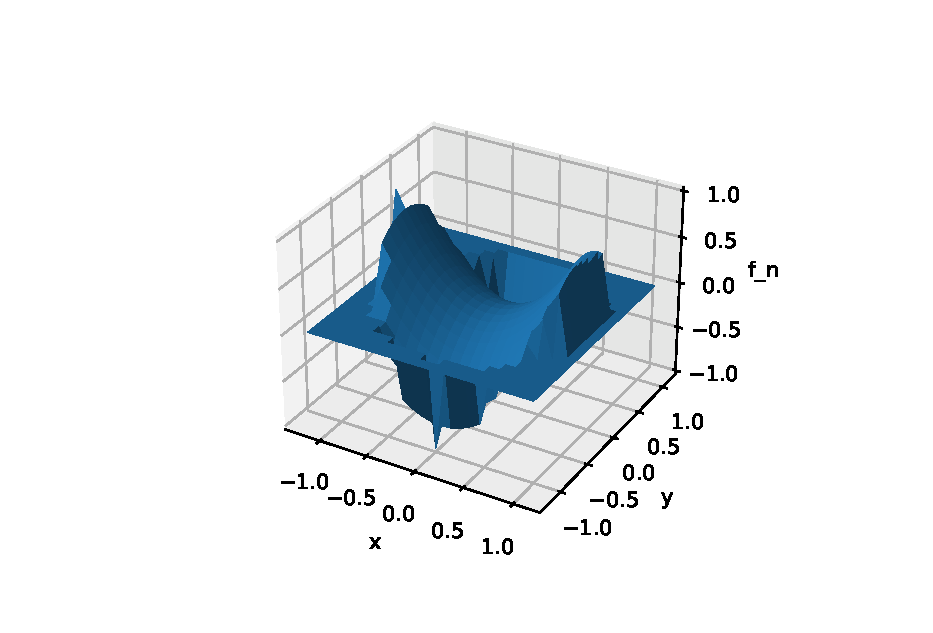
\includegraphics[width=0.7\textwidth]{8_1.eps}\\
	{Рис. 24. Численное решение задачи. }
\end{center}
\begin{center}
	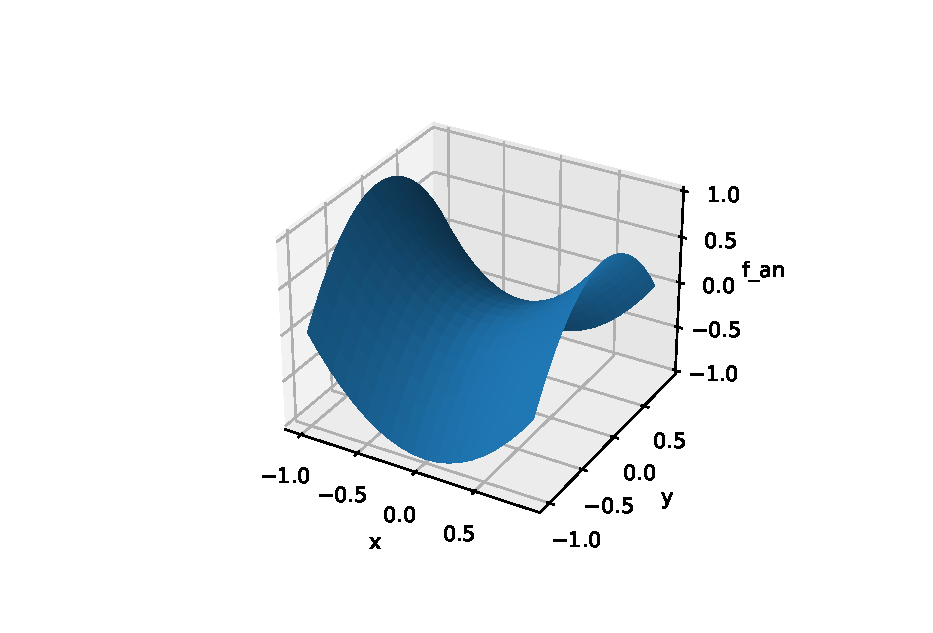
\includegraphics[width=0.7\textwidth]{8_2.eps}\\
	{Рис. 25. Аналитическое решение задачи. }
\end{center}

\newpage

\section{Задание 9}
\subsection{Постановка задачи}
Рассмотреть два вида процессов:
\begin{itemize}
	\item [\textbullet] Винеровский процесс $W(t), t \in [0,1], W(0) = 0.$
	\item [\textbullet] Процесс Орштейна-Уленбека $X(t),t\in [0,1], X(0) = X_0$, то есть стационарный марковский гауссовский процесс. Начальное значение $X_0$ генерируется случайным образом так, чтобы полученный процесс был стационарным.
\end{itemize}
Для данных гауссовских процессов
\begin{enumerate}
	\item Найти ковариационную функцию и переходные вероятности. 
	\item Моделировать независимые траектории процесса с данными переходными вероятностями методом добавления разбиение отрезка.
	\item Построить график траектории, не соединяя точки ломаной, с целью получения визуально непрерывной линии.
\end{enumerate}
\subsection{Решение}
\subsubsection{Винеровский процесс}
\begin{opr}
	Пусть дано вероятностное пространство $(\Omega, \mathcal{F},\mathbb{P}).$ Параметризованное семейство $\{ W_t \}_{t \in T}$ случайных величин
	\[ W_t(\cdot): \Omega \rightarrow \mathbb{R}, \ t\in T, \]
	где $T \subset [0,+\infty)$ интерпретируется как временной интервал, называется случайным процессом.
\end{opr}
\begin{opr}
	Пусть дан случайный процесс $\{W_t \}_{t \in T}$. Тогда он называется гауссовским, если для любых $t_0,t_1,\dots,t_n \in T$ случайный вектор $(W_{t_1},W_{t_2},\dots, W_{t_n})$ имеет многомерное нормальное распределение.
\end{opr}
Определим винеровский процесс как гауссовский процесс в отрезке $[0,1]$ со средним 0 и ковариационной функцией $cov(W(t_i),W(t_j)) = \min (t_i,t_j).$\\
Основные свойства винеровского процесса:
\begin{itemize}
	\item $W_0 = 0$ почти наверное;
	\item $W_t$ является непрерывной функцией от $t$;
	\item Приращения функции $W(t)$ независимы и имеют нормальное распределение со средним равным 0: $W_t - W_s \sim \mathcal{N}(0,1), \ s < t.$
\end{itemize}
Определим плотность $n$-мерного нормального распределения с невырожденной ковариационной матрицей.
\begin{opr}
	Пусть $x$ --- $n$-мерный вектор и $x \sim \mathcal{N}(m_x,R_x)$. Тогда его плотность имеет вид
	\[ p(x) = \frac{1}{(2\pi)^{\frac{n}{2}}\sqrt{|R_x|}}e^{-\frac{1}{2}(x - m_x)^TR_x^{-1}(x - m_x)}, \]
	где $R_x$ --- ковариационная матрица.
\end{opr}
Смоделируем винероский процесс методом деления отрезка $[0,1]$, в отношении $\alpha$, исходя из следующих соображений:
\begin{enumerate}
	\item В начальный момент времени $W_{t_0} = 0$, по определению;
	\item Генерируем $W_{t_1} = W_{t_1} - W_{t_0} \sim \mathcal{N}(0,1)$;
	\item Рассмотрим отрезок $[t_1,t_2]$, его внутреннюю точку $t = t_1 + \alpha(t_2 - t_1)$ и условную плотность
	\[ p_{W_t}(x|W_{t_1} = x_1,W_{t_2} = x_2) = \frac{p_{W_{t_1},W_t,W_{t_2}}(x_1,x,x_2)}{p_{W_{t_1},W_{t_2}}(x_1,x_2)}. \]
	Обозначим векторы $\overline{x} = (x_1,x,x_2)^T$ и $\tilde{x} = (x_1,x_2)^T$ и рассмотрим плотности вероятностей этих векторов:
	\[ p_{W_{t_1},W_t,W_{t_2}} = \frac{1}{(2\pi)^\frac{3}{2}\sqrt{|R_1|}}e^{-\frac{1}{2}\overline{x}^TR_1^{-1}\overline{x}}, \]
	\[ p_{W_{t_1},W_{t_2}} = \frac{1}{(2\pi)\sqrt{|R_2|}}e^{-\frac{1}{2}\tilde{x}^TR_2^{-1}\tilde{x}}, \]
	где $R_1,R_2$ --- соответствующие матрицы ковариаций. Так как ковариационная функция имеет вид $k(s,t) = \min (s,t)$, то находим выражения для $R_1$ и $R_2$:
	\[ R_1 = \begin{pmatrix}
	t_1 & t_1 & t \\
	t_1 & t & t \\
	t_1 & t & t_2
	\end{pmatrix},   \]
		\[ R_2 = \begin{pmatrix}
	t_1 & t_1  \\
	t_1 & t_2
	\end{pmatrix}.  \]
	Вычислим определители и обратные матрицы для $R_1$ и $R_2$:
	\[ R_1^{-1} = \begin{pmatrix}
	  \frac{t}{t_1(t - t_1)}& -\frac{1}{t - t_1} & 0\\
	  -\frac{1}{t - t_1}&  \frac{t_2 - t_1}{(t_2 - t)(t - t_1)}& -\frac{1}{t_2 - t} \\
	  0& -\frac{1}{t_2 - t} & \frac{1}{t_2 - t}
 	\end{pmatrix}, \]
 	\[ R_2^{-1} \begin{pmatrix}
 	\frac{t_2}{t_1(t_2 - t_1)}& -\frac{1}{t_2 - t_1} \\
 	-\frac{1}{t_2 - t_1}& \frac{1}{t_2 - t_1}
 	\end{pmatrix}. \]
 	\[ |R_1| = t_1t_2t + t_1^2t - t_1t^2 - t_1^2t_2; \ |R_2| = t_1t_2 - t_1^2. \]
 	Получим:
 	\[ p_{W_t}(x|W_{t_1} = x_1, W_{t_2} = x_2) = \frac{1}{\sqrt{2\pi\alpha(1 - \alpha)(t_2 - t_1)}} e^{-\frac{(x - ((1 - \alpha)x_1 + \alpha x_2))^2}{2\alpha(1 - \alpha)(t_2 - t_1)}}. \]
\end{enumerate}
\subsubsection{Процесс Орштейна-Уленбека}
\begin{opr}
	Случайный процесс $\{W_t \}_{t \in T}$ называется стационарным, если конечномерные распределения инвариантны относительно сдвига времени.
\end{opr}
\begin{opr}
	Гауссовский процесс $\{ W_t\}_{t \in T}$ называется процессом Орнштейна-Уленбека, если он являетс стационарным и марковским.
\end{opr}
Из стационарности процесса Орнштейна-Уленбека следует, что
\[ \mathbb{E}W_t = a, \ \ R(t,s) = R(|t - s|).  \]
Без ограничений общности положим $a = 0$.\\
Обозначим $\mathbb{D}W_t = \sigma^2$, тогда $R(t,s)$ представима в виде $R(t,s) = \sigma^2 \rho(s,t),$ где $\rho(s,t)$ --- коэффициент корреляции.
\begin{theorem}
	Для того чтобы последовательность $W_1,\dots,W_n$ нормально распределенных случайных величин была марковской, необходимо и достаточно, чтобы 
	\[ \rho_{j,k} = \rho_{j,i}\rho_{i,k} \ \forall i,j,k: j \leq i < k \leq n, \]
	где $\rho_{i,j}$ --- коэффициент корреляции случайных величин $W_i$ и $W_j$.
\end{theorem}
Доказательство представлено в [7] report \\
В силу того, что процесс $W_t$ является марковским, получаем, что
\begin{equation}
\rho(s,t) = \rho(s,\tau)\rho(\tau,t).
\end{equation}
Поскольку $R(s,t) = R(|s - t|)$, то $\rho(s,t) = \rho(s - t).$ Тогда, введя замену переменных
\[ x = s - \tau, \]
\[ y = \tau - t, \]
преобразуем выражение(4) к выражению
\[ \rho(x + y) = \rho(x)\rho(y). \]
\begin{theorem}
	Пусть функция $u(t)$ определена при $t > 0$ и ограничена на каждом конечном интервале. Если $u(t)$ удовлетворяет соотношению $u(t + s) = u(t)u(s)$, то или $u(t) \equiv 0$, или $u(t) = e^{-\lambda t}$, где $\lambda$ --- некоторая положительная константа.
\end{theorem}
Доказательство представлено в [4]\\
Если $\rho(t) \equiv 0$, то $cov(W_t,W_s) = 0$, что равносильно тому, что $W_t$ независимы в совокупности (так как процесс гауссовский), поэтому моделирование процесса Орнштейна-Уленбека заключается в моделировании случайных величин, имеющих распределение $N(a,\sigma^2)$. \\
Рассмотрим случай $\rho(s,t) = e^{-\lambda|s - t|}, \lambda > 0.$ Ковариационная функция процесса Орнштейна-Уленбека имеет вид
\[ R(s,t) = \sigma^2e^{-\lambda|s-t|}. \]
Найдем переходную плоскость
\[ p_{W_t}(x1|W_s = x_2) = \frac{p_{W_t,W_s}(x_1,x_2)}{p_{W_s}(x_2)}.\]
Поскольку $W_t$ --- гауссовский процесс, то 
\[ p_{W_t,W_s}(x_1,x_2) = \frac{1}{2\pi|C|^{\frac{1}{2}}}\exp\bigg\{ -\frac{1}{2}(x,C^{-1}x) \bigg\}, \]
\[ p_{W_s}(x_2) = \frac{1}{\sqrt{2\pi}\sigma}\exp \bigg\{-\frac{x_2^2}{2\sigma^2}  \bigg\}, \]
где $x = (x_1,x_2)$. Ковариационная матрица $C$ имеет вид
\[ C = \begin{pmatrix}
\sigma^2 & R(t,s) \\
R(t,s) & \sigma^2
\end{pmatrix}. \]
Тогда 
\[ |C| = \sigma^4 - R^2(t,s), \ C^{-1} = \frac{1}{|C|}\begin{pmatrix}
\sigma^2 & -R(t,s) \\
-R(t,s) & \sigma^2
\end{pmatrix}. \]
Поэтому
\[p_{W_t}(x_1|W_s = x_2) = \frac{1}{(2\pi(\sigma^2 - \frac{R^2(s,t)}{\sigma^2}))^\frac{1}{2}}\exp \Bigg\{ -\frac{(x_1 - \frac{R(t,s)}{\sigma^2}x_2)^2}{2(\sigma^2 - \frac{R^2(t,s)}{\sigma^2})} \Bigg\},   \]
то есть
\[F(W_t| W_s = x_2) \sim \mathcal{N}(x_2e^{-\lambda|t -s|},\sigma^2(1 - e^{-2\lambda|t-s|})). \]
Для непосредственного моделирования процесса рассмотрим (как и в предыдущем случае) случайные величины $W_{t_1},W_{t_2}.$ Мы можем сгенерировать случайную величину $W_t$, где $t_1 < t < t_2$. Будем моделировать $W_t$  способом аналогичным предыдущему заданию. Для упрощения положим, что $\alpha = 1/2.$ Найдем условную вероятность:
\[ p_{W_t}(x|W_{t_1} = x_1, W_{t_2} = x_2) = \frac{p_{W_{t_1}W_tW_{t_2}}(x_1,x,x_2)}{p_{W_{t_1}}p_{W_{t_2}}},  \]
где $t = \frac{t_1 + t_2}{2},$ поскольку $W_t$ --- гауссовский
\[ p_{W_{t_1}W_tW_{t_2}}(x_1,x,x_2) = \frac{1}{(2\pi)^\frac{3}{2}|R_1|^\frac{1}{2}}\exp\bigg\{-\frac{1}{2}(x_1,x,x_2)^TR_1^{-1}(x_1,x,x_2)\bigg\}, \]
\[p_{W_{t_1}}p_{W_{t_2}} = \frac{1}{2\pi|R_2|^\frac{1}{2}}\exp\bigg\{-\frac{1}{2} (x_1,x_2)^TR_2(x_1,x_2) \bigg\}  \]
где 
\[ R_1 = \sigma^2 \begin{pmatrix}
1 & e^{-\lambda(t_2 - t_1)} & e^{-\lambda(t_2 - t_1)}  \\
e^{-\lambda(t_2 - t_1)}  & 1& e^{-\lambda(t_2 - t_1)}  \\
e^{-\lambda(t_2 - t_1)}  & e^{-\lambda(t_2 - t_1)}  & 1
\end{pmatrix}, R_2 = \sigma^2\begin{pmatrix}
1 & e^{-\lambda(t_2 - t_1)} \\
e^{-\lambda(t_2 - t_1)}  & 1
\end{pmatrix} \]
Используя символьные вычисления получим
\[ W_t \sim N\bigg( (x_1 + x_2)\frac{e^{-\frac{\lambda(t_2 - t_1)}{2}}}{1 + e^{-\lambda(t_2 - t_1)}}, \sigma^2 \frac{1 - e^{-\lambda(t_2 - t_1)}}{1 + e^{-\lambda(t_2 - t_1)}} \bigg) \]
В качестве начальный значений возьмем $W_0 \sim N(0,\sigma^2), W_1 \sim N(x_0e^{-\lambda T},\sigma^2(1 - e^{-2\lambda T})).$
\subsection{Примеры работы программы}
\begin{center}
	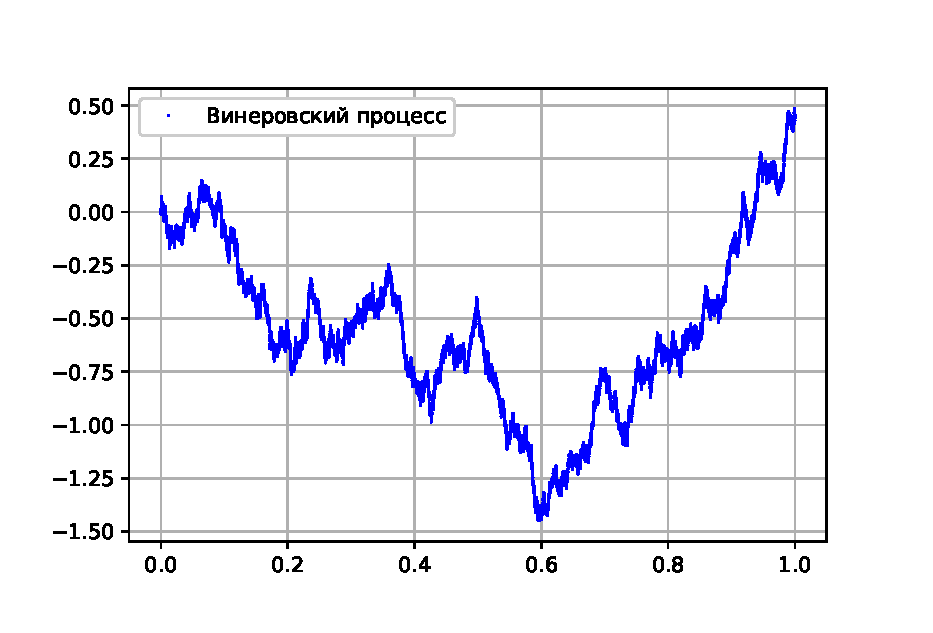
\includegraphics[width=0.7\textwidth]{9_1.eps}\\
	{Рис. 26. Демонстрация винеровского процесса. }
\end{center}
\begin{center}
	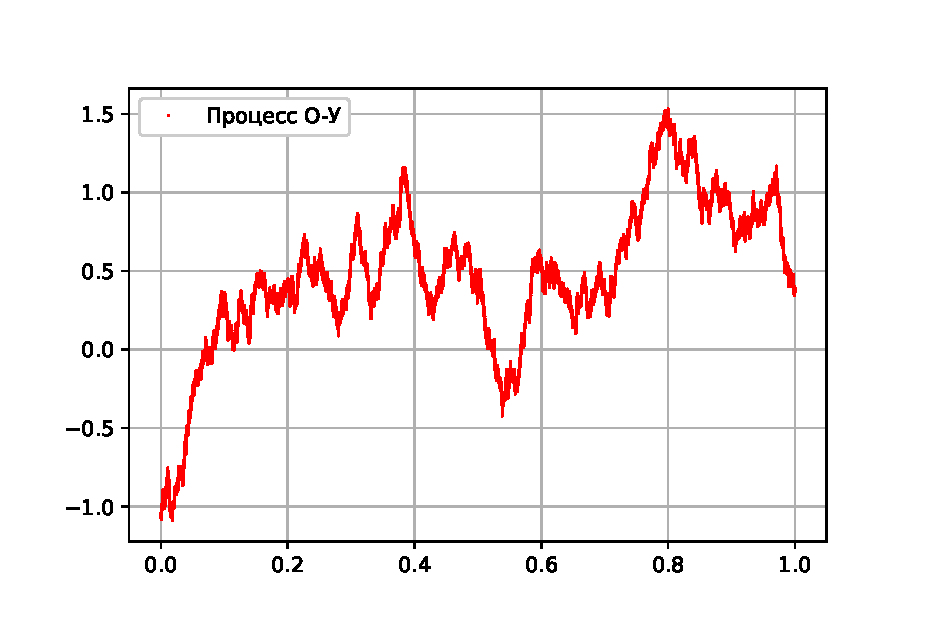
\includegraphics[width=0.7\textwidth]{9_2.eps}\\
	{Рис. 27. Демонстрация процесса Орнштейна-Уленбека. }
\end{center}

\newpage

\section{Задание 10}
\subsection{Постановка задачи}
Провести фильтрацию одномерного процесса Орнштейна-Уленбека:
\begin{enumerate}
	\item Используя генератор белого шума, добавить случайную ошибку с известной дисперсией к реализации процесса Орнштейна-Уленбека.
	\item При помощи одномерного фильтра Калмана оценить траекторию процесса по зашумленному сигналу. Параметры процесса и белого шума считать известными.
	\item Рассмотреть случай, когда шум
	\begin{itemize}
		\item Является гауссовским.
		\item Имеет распределение Коши.
	\end{itemize}
\end{enumerate}
\subsection{Решение}
\subsubsection{Добавлении случайной ошибки}
\begin{opr}
	Дискретным белым шумом называется последовательность $\varepsilon_1,\dots,\varepsilon_n,\dots$ независимых одинаково распределенных случайных величин. 
\end{opr}
Рассмотрим соотношение

\[ x_{k+1} = f(x_k) + \omega(k),\]
где $\omega(k)$ --- случайная помеха, $x_k,\omega(k)$ независимы, $f(x_k) = \mathbb{E}(x_{k+1}|x_k).$ Пусть рассматривается марковский процесс, тогда совместная плотность по всем моментам времени
\begin{eqnarray*}
	p(x_k,\dots,x_0) = p(x_k|x_{k-1},\dots,x_0)\cdot p(x_{k-1}|x_{k-2},\dots,x_0) \cdot \dots \cdot p(x_1|x_0)\cdot p(x_0) = \\
	= \{\text{марковский процесс}\} = p(x_k|x_{k-1})\cdot p(x_{k-1}|x_{k-2})\cdot \dots \cdot p(x_1|x_0)\cdot p(x_0).
\end{eqnarray*}
Обратим внимание, что в случае, когда шум имеет распределение Коши, фильтрацию провести не получится, потому что распределение Коши не имеет математического ожидания. Далее будем рассматривать случай, когда шум является гауссовским.
\subsubsection{Фильтр Калмана}
Рассмотрим линейное стохастическое уравнение
\[ x_{k+1} = A_kx_k + \omega_k. \]
Поскольку случайные величины гауссовские, то для их полного описания достаточно знать их первые и вторые моменты.\\
Пусть имеет следующую систему:
\begin{equation}
 \begin{cases}
x_{k+1} = A_kx_k + \omega_k, \\
y_{k+1} = C_{k+1}x_{k+1} + v_{k+1},
\end{cases} 
\end{equation}
причем $x_0,\omega_0,\dots,\omega_{N-1},v_0,\dots,v_{n-1}$ независимы в совокупности. $Y_{N-1} = (y_0,\dots,y_{N-1})^T$ --- все наблюдения, а $X_{N-1} = (x_0,\dots,x_{N-1})$ --- исходный процесс, который надо найти. Для это воспользуемся фильтром Калмана, а именно его схемой <<шагаем-мерим>>, общий вид которой совпадает с (5).\\
Обозначим $\mathbb{E}x_0 = \overline{x}_0, \mathbb{D}x_0 = S,\mathbb{E}\omega_k = \mathbb{E}v_k = 0, \mathbb{D}\omega_k = M_k,\mathbb{D}v_k = N_k > 0.$\\
Фильтра Калмана для схемы <<шагаем-мерим>> имеет вид:
\[  
\begin{cases}
\tilde{x}_{k+1|k} = A_k\tilde{x}_{k|k},\\
\tilde{x}_{k+1|k+1} = \tilde{x}_{k+1|k} + R_{k+1}C^T_{k+1}(C_{k+1}R_{k+1|k}C^T_{k+1} + N_{k+1})^{-1}(y_{k+1} - C_{k+1}\tilde{x}_{k+1|k}),\\
R_{k+1|k} = A_kR_{k|k}A^T_k + M_k,\\
R_{k+1|k+1} = R_{k+1|k} - R_{k+1|k}C^T_{k+1}(C_{k+1}R_{k+1|k}C^T_{k+1} + N_{k+1})^{-1}C_{k+1}R_{k+1|k},\\
\tilde{x}_{0|0} = \overline{x}_0,\\
R_{0|0} = S.
\end{cases}
\]
В нашей задаче $x_k$ --- процесс Орнштейна-Уленбека с параметрами $\sigma_W$ и $\lambda, y_{k+1} = x_{k+1} + v_{k+1}$, где $v$ ---  белый шум. Пусть $\sigma_n^2$ --- его дисперсия. Тогда получаем, что $N_k = \sigma_n^2,$ а $C_k = 1$. Осталось найти $A_k$ и $M_k$. Будем считать, что $t_{i+1} - t_i = \Delta t$ независимо от $i$. Так как мы рассматриваем одномерный процесс Орнштейна-Уленбека, то $A_k,C_k$ являются скалярами, и от их транспонирования ничего не меняется. Обозначим $\mathbb{D}x_k = V_k.$ \\
С одной стороны имеем
\[ \mathbb{D}x_{k+1} = A_k^2\mathbb{D}x_k + \mathbb{D}\omega_k = A_k^2 V_k + M_k, \]
\begin{eqnarray*}
cov(x_{k+1},x_k) = \mathbb{E}(x_{k+1},x_k) - \mathbb{E}x_{k+1}\mathbb{E}x_k = \mathbb{E}(A_kx_k^2 + \omega_{k+1}x_k) - A_k(\mathbb{E}x_k)^2 = \\
= \{\mathbb{E}\omega_{k+1} = 0, \omega_{k+1} \text{ и } x_k \text{ независимы} \} = A_k(\mathbb{E}x_k^2 - (\mathbb{E}x_k)^2) = A_k\mathbb{D}x_k = A_kV_k.
\end{eqnarray*}
С другой стороны так как ковариационная функция процесса Орнштейна-Уленбека имеет вид $R(t,s)= \sigma^2_W e^{-\lambda|t-s|},$ то получим следующую систему уравнений:
\[ 
\begin{cases}
A^2_kV_k + M_k = \sigma^2_W,\\
A_kV_k = \sigma^2_We^{-\lambda\Delta t},\\
V_k = \sigma_W^2.
\end{cases}
\]
Получаем, что $V_k = \sigma_W^2, A_k = e^{-\lambda\Delta t},M_k = \sigma^2_W(1 - e^{-2\lambda\Delta t}).$ Обратим внимание, что когда мы в 9 задании вводили процесс Орнштейна-Уленбека, то считали, что $\mathbb{D}x_k = \sigma_W^2$, что согласуется с тем, что мы получили.\\
Следовательно, фильтр Калмана для нашей задачи будет иметь вид:
\[  
\begin{cases}
\tilde{x}_{k+1|k} = e^{-\lambda\Delta t}\tilde{x}_{k|k},\\
\tilde{x}_{k+1|k+1} = \tilde{x}_{k+1|k} + R_{k+1|k}(R_{k+1|k} + \sigma_n^2)^{-1}(y_{k+1} - \tilde{x}_{k+1|k}),\\
R_{k+1|k} = e^{-2\lambda \Delta t} R_{k|k} + \sigma^2_W(1 - e^{-2\lambda \Delta t}),\\
R_{k+1|k+1} = R_{k+1|k} - R_{k+1|k}(R_{k+1|k} + \sigma^2_n)^{-1}R_{k+1|k},\\
\tilde{x}_{0|0} = 0,\\
R_{0|0} = \sigma_W^2.
\end{cases}
\] 
Обозначив $h = R_{k+1|k}(R_{k+1|k} + \sigma^2_n)^{-1}$, получим итоговую систему:
\[  
\begin{cases}
\tilde{x}_{k+1|k} = e^{-\lambda\Delta t}\tilde{x}_{k|k},\\
\tilde{x}_{k+1|k+1} = (1 - h)\tilde{x}_{k+1|k} + hy_{k+1},\\
h =  R_{k+1|k}(R_{k+1|k} + \sigma^2_n)^{-1}, \\
R_{k+1|k} = e^{-2\lambda \Delta t} R_{k|k} + \sigma^2_W(1 - e^{-2\lambda \Delta t}),\\
R_{k+1|k+1} = (1 - h)R_{k+1|k},\\
\tilde{x}_{0|0} = 0,\\
R_{0|0} = \sigma_W^2.
\end{cases}
\]
В данном случае доверительный интервал
\[x_k + k_{1- \frac{\alpha}{2}}[-\sqrt{R_{k|k}},\sqrt{R_{k|k}}]\]
где $k_\alpha$ --- квантиль стандартного нормального распределения.
\subsection{Примеры работы программы}
\begin{center}
	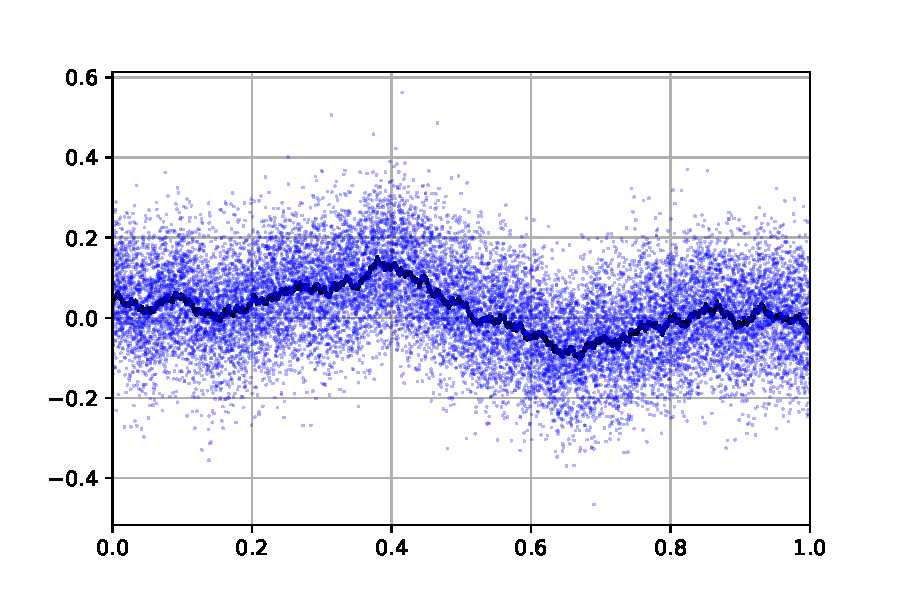
\includegraphics[width=0.7\textwidth]{10_1.pdf}\\
	{Рис. 28. Процесс Орнштейна-Уленбека с гауссовским шумом. }
\end{center}
\begin{center}
	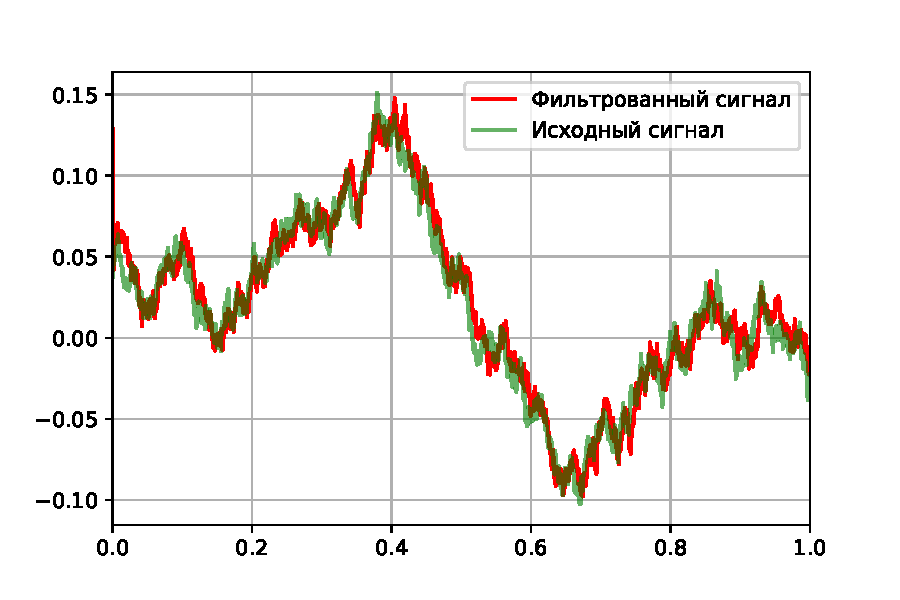
\includegraphics[width=0.7\textwidth]{10_2.pdf}\\
	{Рис. 29. Результат применения работы фильтра Калмана к процессу Орнштейна-Уленбека с гауссовским шумом . }
\end{center}
\begin{center}
	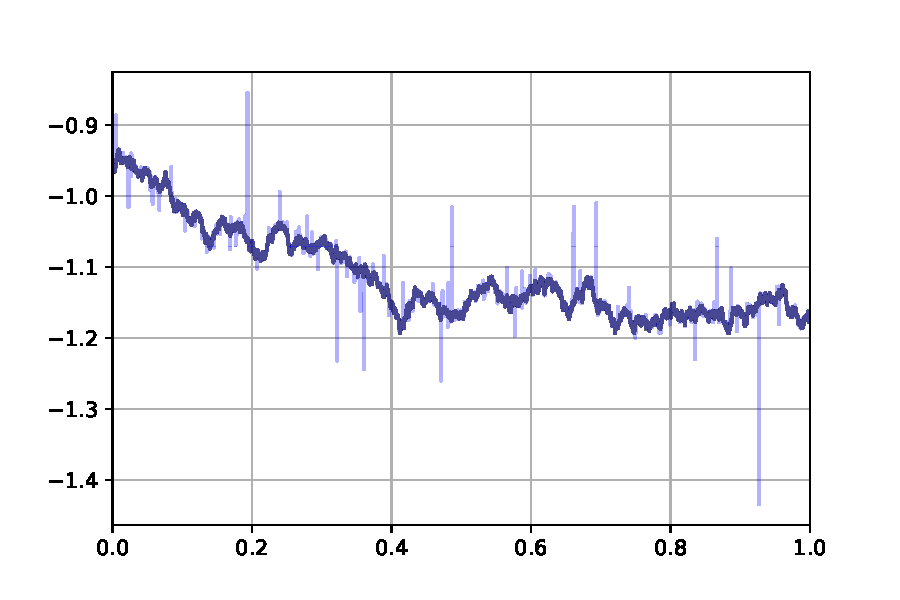
\includegraphics[width=0.7\textwidth]{10_3.pdf}\\
	{Рис. 30. Процесс Орнштейна-Уленбека с шумом, имеющим распределение Коши. }
\end{center}
\begin{center}
	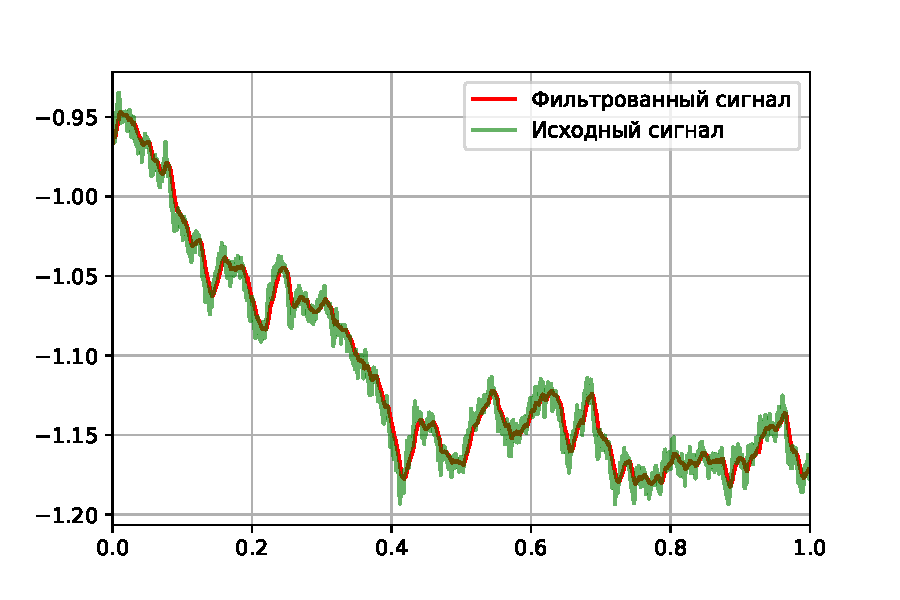
\includegraphics[width=0.7\textwidth]{10_4.pdf}\\
	{Рис. 31. Результат применения работы фильтра Калмана к процессу Орнштейна-Уленбека с шумом, имеющим распределение Коши. }
\end{center}

\newpage

\section{Задание 11}
\subsection{Постановка задачи}
Построить двумерное пуассоновское поле, отвечающее сложному пуассоновскому процессу:
\begin{enumerate}
	\item Первая интерпретация: система массового обслуживания. При этом, первая координата поля --- время поступления заявки в СМО (равномерное распределение), вторая --- время ее обслуживания (распределение $\chi^2$ c 10 степенями свободы).
	\item Вторая интерпретация: система массового обслуживания с циклической интенсивностью $\lambda(1 + \cos(t))$ и единичными скачками. Свести данную задачу моделирования неоднородного пуассоновского процесса при помощи метода Льюиса и Шеддера к моделированию двумерного пуассоновского поля, где первая координата имеет равномерное распределение, а вторая --- распределение Бернулли.
	\item Третья интерпретация: работа страховой компании. Первая координата --- момент наступления страхового случая (равномерное распределение), вторая координата --- величина ущерба (распределение Парето). Поступление капитала по времени линейно со скоростью $c > 0$, начальный капитал $W > 0$.
	\item Для каждой системы  рассмотреть всевозможные случаи поведения системы в зависимости от значения параметров.
\end{enumerate}
\subsection{Решение}
\subsubsection{Первая интерпретация: система массового обслуживания}
Пусть $\lambda$ --- интенсивность пуассоновского поля. Времена поступления заявок генерируются так, что $\Delta t_i = t_i - t_{i-1} \sim Exp(\lambda).$
\begin{opr}
	Распределением $\chi^2$ с $k$ степенями свободы называется распределение суммы квадратов $k$ независимых стандартных нормальных случайных величин.
\end{opr}
Время обслуживания каждой заявки $s_i$ независимы и генерируются как случайные величины с распределением $\chi^2(10)$.\\
Поскольку все заявки обрабатываются последовательно, время окончания обработки заявки, поступившей в момент времени $t_i$ можно найти следующим образом:
\begin{itemize}
	\item если к моменту поступления заявки предыдущая заявка уже обработана, то нужно к времени поступления текущей заявки прибавить время ее обработки:
	\[ Q_i = t_i + s_i. \]
	\item если предыдущая заявка еще не обработана, то нужно прибавить к времени конца обработки предыдущей заявки время обработки текущей:
	\[ Q_i = Q_{i-1} + s_i. \]
\end{itemize}
Обобщая вышесказанное, имеем:
\[ Q_i = t_i + \max (0,Q_{i-1} - t_i) + s_i. \]
Для каждой заявки будем считать количество людей в очереди.
\begin{itemize}
	\item если во время поступления $i-$й заявки очереди не было то положим $n_i = 0$.
	\item если предыдущая заявка еще не обработана, то:
	\[ n_i \neq Q_k: k < i \text{ и } Q_k > t_i, \]
	т.е. количество еще не выполненных к моменту времени $t_i$ заявок.
\end{itemize}
Поскольку время обработки еще одной заявки в среднем равно 10, а средний интервал между поступлениями заявок равен $\mathbb{E}\Delta_i = \frac{1}{\lambda}$, то при $\lambda < 0.1$ очереди практически не будет, а при $\lambda > 0.1$ очередь будет неограниченно расти.
\subsubsection{Вторая интерпретация: система массового обслуживания с циклической интенсивностью и единичными скачками}
Пусть $T_1,\dots,T_n\dots$ --- времена наступления некоторых событий, а $N(t_1,t_2)$ --- количество событий, произошедших в промежуток $[t_1,t_2]$. Заметим, что $T_{n+1} - T_n$ имеет функцию распределения $F(x) = 1 - \exp\{-\Lambda(t + x) - \Lambda(t)\}, x > 0$, где 
\[\Lambda(t) = \int_{0}^{t}\lambda(u)du = \lambda(t + \sin t)\]
неограниченно возрастает с ростом $t$. \\
$T_{n+1}$ распределено как $T_n + F^{-1}(U)$, где $U$ равномерно распределена на $[0,1]$. Заметим, что если записать $U$ как $1-\exp\{-E\}$, где $E$ --- экспоненциальная случайная величина с параметром $\lambda_E = 1$, то $T_{n+1}$ распределена как $\Lambda^{-1}(E + \Lambda(T_n)).$\\
Будем искать обратную функцию $\Lambda^{-1}(y)$ численно, так как аналитически это не представляется возможным $(\Lambda'(t) = \lambda_0(1 + \cos (t))$ почти всюду положительна, то есть функция возрастает). Такой метод моделирования неоднородного процесса Пуассона называется методом Льюиса-Шеддера.\\
Чтобы не искать обратную функцию, можно воспользоваться следующей модификацией метода Льюиса-Шеддера. Пусть имеется переменная $t$, в которой хранится текущее время (но не обязательно событие произошло строго в это время).
\begin{itemize}
	\item На каждом шаге генерируем случайную величину $\xi \sim Exp(2\lambda_0)$.
	\item Прибавляем к переменной $t$ величину $\xi$ и генерируем случайную величину $\eta = Bern(\frac{1 + \cos t}{2}).$
	\begin{itemize}
		\item [---] если она приняла значение 1, то полагаем $T_{i+1} = t$ и $i = i+1$
		\item [---] иначе ничего не делаем и повторяем процесс заново
	\end{itemize}
\end{itemize}
 
\subsubsection{Третья интерпретация: работа страховой компании}
\begin{opr}
	Случайная величина $X$ имеет распределение Парето с параметрами $x_m$ и $k$, если ее функция распределения имеет вид:
	\[ F_X(x) = 1 - \bigg(\frac{x_m}{x}\bigg)^k. \]
\end{opr}
Для моделирования случайной величины, имеющей распределение Парето, снова воспользуемся методом обратной функции.\\
Обратная функция для данной функции распределения имеет вид:
\[ F^{-1}_X(x) = \frac{x_m}{(1 - x)^\frac{1}{k}}. \]
Сгенерируем времена наступления страховых случаев на временном интервал $[0,T]$:
\[ 0 \leq t_1 \leq \dots \leq t_n < T, \]
причем $t_i - t_{i-1} \sim Exp(\lambda), \lambda > 0$ --- интенсивность потока страховых случаев.\\
Величину ущерба $s_i$ страхового случая в момент времени $t$ будем генерировать с помощью распределения Парето с параметрами $x_m$ и $k$. Случайную величину, распределенную по Парето, будем генерировать, воспользовавшись методом обратных функций:
\[ F^{-1}_\xi (y) = \frac{x_m}{(1-x)^\frac{1}{k}}. \]
Учтем, что если $Y \sim U[0,1],$ то и $(1 - Y) \sim U[0,1]$. Тогда случайная величина
\[ X = x_m Y^{-\frac{1}{k}}, \ Y \sim U[0,1] \]
имеет распределение Парето с параметрами $x_m$ и  $k$.\\
Величина капитала компании в момент времени $t$ выражается как
\[ W_t = W_0 + ct - s(t), \]
где $s(t)$ --- сумма величин ущерба страховых случаев, произошедших в моменты времени $t_i$ такие, что $t_i \leq t$. Время разорения --- случайная величина, задаваемая следующим условием:
\[ T = \min \{t > 0| W_t < 0 \}.\]
Выведем зависимость функции $W(t)$ от параметров $\lambda, x_m, k,W_0,c.$ Будем считать, что $k > 1$. Тогда 
\[\mathbb{E}W'(t) = c - \mathbb{E}'s(t) = c - \bigg( \mathbb{\bigg[\sum_{t_i < t}^{}s_i\bigg]} \bigg)' = c - \bigg(\frac{t}{\frac{1}{\lambda}}\mathbb{E}[s_i]\bigg)'=c - \frac{\lambda k x_m}{k -1}.\]
Таким образом:
\begin{itemize}
	\item $c(k-1) > \lambda kx_m$ капитал растет.
	\item $c(k-1) = \lambda kx_m$ система находится в положении равновесия.
	\item $c(k-1) < \lambda kx_m$ капитал уменьшается.
\end{itemize}

\subsection{Примеры работы программы}
\begin{center}
	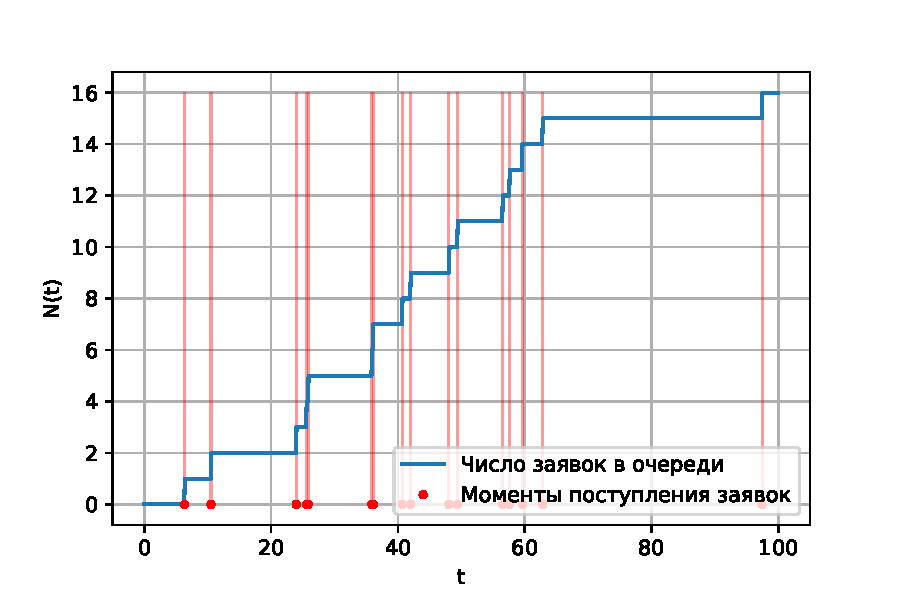
\includegraphics[width=0.7\textwidth]{11_1.pdf}\\
	{Рис. 32. Моделирование СМО. }
\end{center}
\begin{center}
	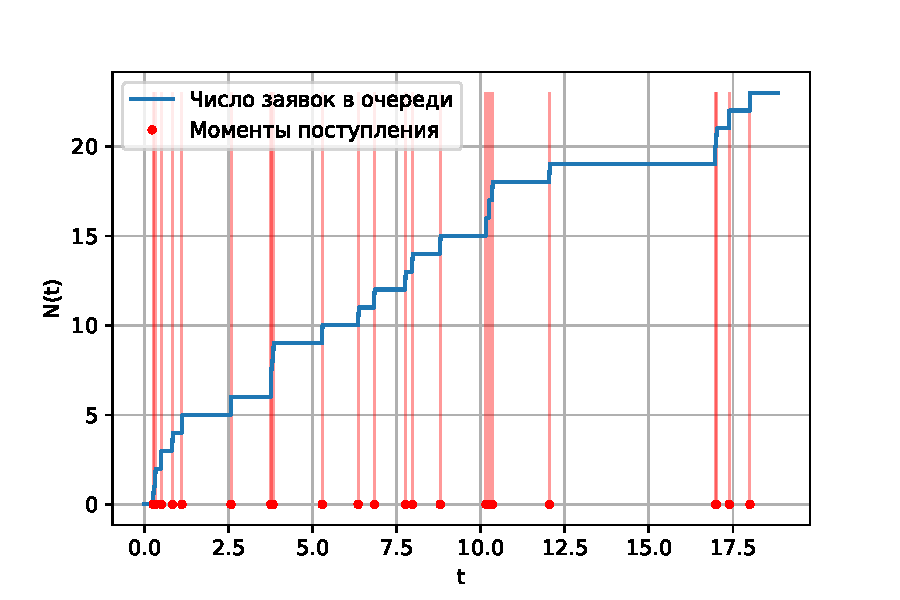
\includegraphics[width=0.7\textwidth]{11_2.pdf}\\
	{Рис. 33. Моделирование СМО с циклической активностью. }
\end{center}
\begin{center}
	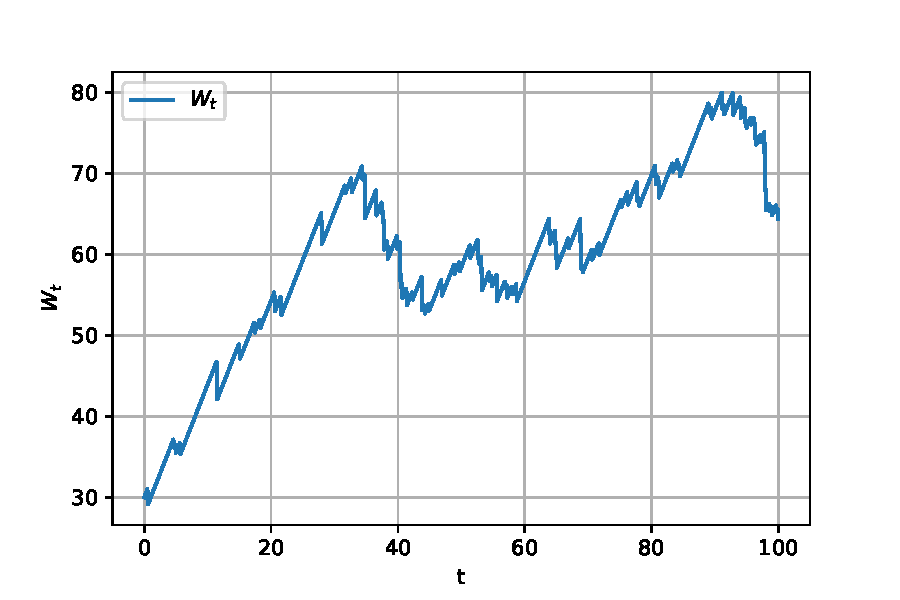
\includegraphics[width=0.7\textwidth]{11_3.pdf}\\
	{Рис. 34. Моделирование работы страховой компании. }
\end{center}

\newpage
\section{Список литературы}
$[1]$ Смирнов С.Н. Лекции по курсу <<Стохастический анализ моделирование>>, 2021.\\ \\
$[2]$ Ширяев А.Н. Вероятность, Наука. М.:1989. \\ \\
$[3]$ Кропачёва Н.Ю., Тихомиров А.С. Моделирование случайных величин: Метод указания, НовГУ им. Ярослава Мудрового, 2004 \\ \\
$[4]$ Феллер В. Введение в теорию вероятностей и её приложения, в 2---х томах. Т.1, М., Мир, 1984.
\end{document} 

	